\documentclass[11pt]{cernrep}
\usepackage{graphicx,epsfig}
\bibliographystyle{lesHouches}


\usepackage{heppennames2}
\usepackage{cernunits}
\usepackage{hepparticles}

\renewcommand{\arraystretch}{1.6}



\begin{document}



\section{NLO EW technical and physics comparisons%
\protect\footnote{Section
    coordinators: V.~Ciulli, A.~Denner} 
$^{,}$~\protect\footnote{Contributing authors: 
M. Chiesa, 
%V. Ciulli, 
%A.~Denner, 
R. Frederix,  
%N.~Greiner,
L.~Hofer,
S.~Kallweit,
J.M.~Lindert,
P.~Maierh\"ofer,
A.~Marini, 
G.~Montagna, 
M.~Moretti, 
O.~Nicrosini, 
D.~Pagani,
F.~Piccinini,
S.~Pozzorini,
M.~Sch\"onherr, 
E.~Takasugi,
%J.~Thompson,
S.~Uccirati, 
M.A. Weber,
M.~Zaro}}


Adequate predictions for scattering processes at particle colliders
such as the LHC require the inclusion of next-to-leading order (NLO)
perturbative corrections of the strong and electroweak (EW) interactions.
For the calculation of NLO QCD corrections the automation has been
established, and several tools exist
\cite{Hahn:1998yk,Arnold:2008rz,Berger:2008sj,Becker:2010ng,
  Badger:2010nx,Hirschi:2011pa,Bevilacqua:2011xh,Cullen:2011ac,Cascioli:2011va}.
On the other hand, the automation of NLO EW corrections has just
started, and only a few tools are available
\cite{Actis:2012qn,Kallweit:2014xda,Frixione:2014qaa,Chiesa:2015mya}.
In this section we review the status of the existing tools for the
automated calculation of EW one-loop amplitudes and provide a
comparison of some of them for specific processes. In addition,
we also show a comparison of the Sudakov approximation for the EW
corrections as implemented in {\sc Alpgen} \cite{Mangano:2002ea}
%and {\sc Sherpa}~\cite{Gleisberg:2007md,Gleisberg:2008ta} 
with complete NLO calculations. 
%
Finally, we present a comparison of theoretical predictions from
various codes with experimental results from CMS for the ratio of the
associated production of a $\PZ/\gamma^*$ or an on-shell photon with
additional jets as a function of the transverse momentum of the
vector boson.
 

\subsection{Codes for the automated calculation of electroweak NLO corrections}

\subsubsection*{\sc Recola}

{\sc Recola} is a Fortran95 computer program for the automated
generation and numerical computation of scattering amplitudes in the
full Standard Model (SM) (including QCD and the EW sector) at tree
and one-loop level. It is based on a one-loop generalization of
Dyson--Schwinger recursion relations \cite{vanHameren:2009vq} and
allows to generate one-loop amplitudes for (in principle) arbitrary
decay and scattering processes in the SM with 
particular emphasis on high particle multiplicities. Counterterms
\cite{Denner:1991kt} and rational terms \cite{Garzelli:2009is} are
included via dedicated tree-level Feynman rules. {\sc Recola} was the
first automated tool to calculate EW NLO corrections
\cite{Actis:2012qn}.

{\sc Recola} provides numerical results for scattering amplitudes in
the 't~Hooft--Feynman gauge. 
Dimensional regularization is used for ultraviolet singularities,
while collinear and soft singularities can be treated either in
dimensional or in mass regularization. {\sc Recola} is interfaced to
the {\sc Collier} library \cite{Denner:2014gla,collier-hepforge} for
the fast and numerically stable calculation of one-loop tensor
integrals. For renormalization, apart from
the traditional on-shell scheme~\cite{Denner:1991kt}, {\sc Recola} in
particular features its generalization to the complex-mass scheme~\cite{Denner:2005fg}.
{\sc Recola} further supports the $G_\mu$, the $\alpha(0)$ and the
$\alpha(M_{\PZ})$ scheme for the renormalization of the
electromagnetic coupling constant, and a dynamical
$N_{\mathrm{f}}$-flavour scheme for the strong coupling constant. Internal resonant particles can be
treated in the complex-mass scheme. Moreover,
resonant contributions can be consistently isolated such that matrix
elements involving specific intermediate resonances can be calculated. The
calculation of squared amplitudes, summed over spin and colour, is
supported at leading order (LO), NLO, and for loop-induced processes.
Besides the calculation of complete tree-level and one-loop results,
{\sc Recola} allows to select or discard specific orders of $\alpha_s$
(and thus also of $\alpha$) in all computed objects, such as in the
amplitudes, in the square of the Born amplitude or in the interference
of the Born with the one-loop amplitude.  Moreover, the code allows
the computation of colour- and spin-correlated LO squared amplitudes
required for dipole subtraction \cite{Catani:1996vz,Catani:2002hc}.
%Recola is publicly available for download via hepforge \cite{recola-hepforge}.

For the calculation of physical cross sections {\sc Recola} has to be
interfaced to a Monte Carlo code or a multi-purpose event generator;
such interfaces are presently being developed.  Together with private
Monte Carlo integrators, {\sc Recola} has been used for the computation
of EW corrections to $\Pp\Pp \to \Pl^+ \Pl^-{\rm j j},
\nu_{\Pl}\bar\nu_{\Pl}{\rm j j} $ \cite{Denner:2014ina} and the QCD
corrections to $\Pp\Pp\to\Pe^+\nu_{\Pe}
\mu^-\bar{\nu}_\mu\PQb\bar{\PQb}\PH$ \cite{Denner:2015yca}.




\subsubsection*{{\sc Sherpa/Munich+OpenLoops}}


The frameworks {\sc Munich + OpenLoops} and {\sc Sherpa + OpenLoops}
automate the full chain of operations -- from process definition to
collider observables -- that enter NLO QCD+EW simulations at parton
level.
%
The relevant scattering amplitudes at NLO QCD are publicly available
in the form of an automatically generated library
\cite{openloops-hepforge} that supports all interesting LHC processes
(more than one hundred processes), can be easily extended upon user
request and will be extended to NLO EW soon.
%
The recently achieved automation of EW
corrections~\cite{Kallweit:2014xda,Kallweit:2015dum} is based on the
well established QCD implementations and allows for NLO QCD+EW
simulations for a vast range of SM processes, up to high particle
multiplicity, at current and future colliders.
%
To be precise, the new implementations allow for NLO calculations at
any given order $\alpha_s^n\alpha^m$, including all relevant QCD--EW
interference effects.  Full NLO SM calculations that include all
possible $\mathcal{O}(\alpha_s^{n+k} \alpha^{m-k})$ contributions to a
certain process are also supported.


In these frameworks virtual amplitudes are provided by the {\sc OpenLoops}
program~\cite{openloops-hepforge}, which is based on the Open Loops algorithm~\cite{Cascioli:2011va} --
a fast numerical recursion for the evaluation of one-loop scattering 
amplitudes.
%
The extension to NLO EW corrections required the
implementation of all $\mathcal{O}(\alpha)$ EW Feynman rules in the
framework of the numerical Open Loops recursion including counterterms
associated with so-called $R_2$ rational parts~\cite{Garzelli:2009is}
and with the on-shell renormalization of UV
singularities~\cite{Denner:1991kt}.  Additionally, for the treatment
of heavy unstable particles the complex-mass
scheme~\cite{Denner:2005fg} has been implemented in a fully general
way.
%
Combined with the {\sc Collier} tensor-reduction library
\cite{Denner:2014gla}, which implements the Denner--Dittmaier
reduction techniques~\cite{Denner:2002ii,Denner:2005nn} and the scalar
integrals of Ref.~\cite{Denner:2010tr}, or with {\sc
  CutTools}~\cite{Ossola:2007ax}, which implements the OPP
method~\cite{Ossola:2006us}, together with the {\sc OneLOop}
library~\cite{vanHameren:2010cp}, the employed recursion permits to
achieve very high CPU performance and a high degree of numerical
stability.


All remaining tasks, i.e.\ the bookkeeping of partonic subprocesses,
phase-space integration and the subtraction of QCD and QED
bremsstrahlung are supported by the two independent and fully
automated Monte Carlo generators {\sc Munich}~\cite{munich} and {\sc
  Sherpa}~\cite{Gleisberg:2007md,Gleisberg:2008ta}.  The first one,
{\sc Munich}, is a fully generic and very fast parton-level Monte
Carlo integrator. {\sc Sherpa} is a particle-level Monte Carlo
generator providing all stages of hadron-collider simulations,
including parton showering, NLO matching, multi-jet merging,
hadronization and underlying event simulations.  For tree amplitudes,
with all relevant colour and helicity correlations, {\sc Munich}
relies on {\sc OpenLoops}, while {\sc Sherpa} generates them
internally with {\sc Amegic++} \cite{Krauss:2001iv} and {\sc Comix}
\cite{Gleisberg:2008fv}.
%
For the cancellation of infrared singularities both Monte Carlo tools,
{\sc Munich} and {\sc Sherpa}, employ the dipole-subtraction
scheme~\cite{Catani:1996vz,Catani:2002hc} and its extension to EW
corrections~\cite{Dittmaier:1999mb,Dittmaier:2008md}.  Both codes were
extensively checked against each other, and sub-permille level
agreement was found. The implementation of parton-shower matching and
multi-jet merging including NLO EW effects is available in an
approximate way~\cite{Kallweit:2015dum}, while a fully consistent
implementation is under way.

Employing the described frameworks in Ref.~\cite{Kallweit:2014xda} the
simulation of $\PW+1,2,3$ jet production at NLO EW+QCD was presented.
In order to make the calculation of the process with the highest jet
multiplicity feasible, it was important to factorize these processes
into a production part and into a decay part. At the NLO EW level this
required a careful implementation of the narrow-width approximation in
order to control numerical stability given the appearance of
pseudo-resonances for two or more associated jets. It was found that
$V$ + multijet final states feature genuinely different EW effects as
compared to the case of $V + 1$ jet. Subsequently in
Ref.~\cite{Kallweit:2015dum} NLO QCD+EW simulations were presented for
$\PZ+{}$jets and $\PW^{\pm}+{}$jets production including off-shell leptonic
decays and multijet merging with up to two jets within the MEPS@NLO
framework of the {\sc Sherpa} Monte Carlo program.


\subsubsection*{{\sc\small MadGraph5\_\-aMC@NLO}}



%\begin{table}[t]
%\renewcommand{\arraystretch}{1.5}
%\scriptsize
%    %%% RESULTS FOR TTH: RELATIVE CORRECTIONS
%    \centering
%    \begin{tabular}{c|ccccc}
%        $\PQt\bar\PQt\PH$      & inclusive & $p_{\mathrm{T}}(i) > 200\,{\rm GeV}$ & $p_{\mathrm{T}}(i) > 400\,{\rm GeV}$ & $p_{\mathrm{T}}(\PH) > 500\,{\rm GeV}$ & $|y(\PQt)| > 2.5$\\
%        \hline
%        $\sigma_{{\rm LO~QCD}}$, $\alpha_s^2 \alpha$ ~[\rm pb]         & $  3.617 \cdot 10^{-1} $ &$  1.338 \cdot 10^{-2} $ &$3.977 \cdot 10^{-4}$&  $2.013  \cdot 10^{-3} $ &  $4.961  \cdot 10^{-3} $ \\  
%        \hline  \hline
%         $\delta(X) ~[\%]$  \\
%           \hline  \hline
%        ${\rm NLO~QCD}$ , $\alpha_s^3 \alpha$         &  $ 29.7   $ &$   24.2  $ & $11.3$ & $38.8$ & $38.0$\\  
%                ${\rm NLO~QCD} $ (6f-PDFs), $\alpha_s^3 \alpha$         &  $ 28.9   $ &$   23.4  $ & $9.6$ & $37.8$ & $37.5$\\  
%        \hline
%        ${\rm LO~QCD}$, $\alpha_s \alpha^2$          & $    1.2  $ &$    2.8 $ &$    5.7 $  &$    3.0 $ &$    12.0 $\\  
%        ${\rm LO~QCD}$, $\alpha_s \alpha^2$  
%                            no $\gamma$   & $   -0.4  $ &$   -0.2  $ &$   -0.1 $ &$   -0.1 $ &$   -0.1 $ \\  
%        \hline
%        ${\rm NLO~EW}$, $\alpha_s^2 \alpha^2$         & $   -1.2$ &$   -8.2  $   & $-13.8$ & $-10.6$ & $+0.2 $ \\  
%        ${\rm NLO~EW}$, $\alpha_s^2 \alpha^2$  
% no $\gamma$  & $   -1.4 $ &$   -8.5 $ & $-13.9$ & $-11.6$ & $+0.5$ \\  
%    \end{tabular}
%    \caption{LO QCD cross sections and relative corrections for different cuts.}
%    \label{tab:ttH_rel}
%\end{table}


The results presented in Section~\ref{sec:comp;ew} have been obtained
via an extension of the public code {\sc\small
  MadGraph5\_\-aMC@NLO}~\cite{Alwall:2014hca} that allows to
automatically calculate also NLO EW corrections. This version of the
code is, at the moment, private and has already been used for the
calculation of NLO QCD and EW corrections to the hadroproduction of a
top-quark pair in association with a heavy boson
\cite{Frixione:2014qaa, Frixione:2015zaa}.

The automation of the NLO QCD and EW corrections for a generic SM
process has required major improvements for all the building blocks of
the {\sc\small MadGraph5\_\-aMC@NLO} code
\cite{Frederix:2009yq,Hirschi:2011pa}.  The generation of the
amplitudes and matrix elements at LO and NLO accuracy for the combined
expansion in powers of $\alpha_s$ and $\alpha$ has been lengthly
discussed in Refs.~\cite{Alwall:2014hca, Frixione:2014qaa}. The code
at the moment is able to automatically calculate all the possible
perturbative orders stemming from tree-level amplitudes and their
interference with one-loop amplitudes, for any SM process.
Moreover, it is possible to select any combination of perturbative
orders. Thus, all the necessary $R_2$ and UV counterterms have been
calculated both in the complex-mass scheme and with real masses
and on-shell renormalization conditions for unstable particles. These
counterterms are part of the so-called NLO UFO models
\cite{Degrande:2011ua}, which is the general format used in {\sc\small
  MadGraph5\_\-aMC@NLO} for importing Feynman rules of a given
Lagrangian. In the case of the SM at NLO, two different UFO models
have been created in order to calculate EW corrections
respectively in the $\alpha(m_{\PZ})$ or $G_{\mu}$~scheme.

The subtraction of infrared divergences and the integration over the
Born-like and real-emission phase space is automatically performed for
any process by extending the framework described in
Refs.~\cite{Alwall:2014hca,Frederix:2009yq}, taking into account all
the EW-QCD IR divergences appearing at any perturbative order that
enter into NLO predictions.

At the moment, NLO corrections for massive-only final states can be
automatically calculated by running a code that can be generated in
{\sc\small MadGraph5\_\-aMC@NLO} via few commands of the form:%
\footnote{These are representative commands, the future public version
  of the code may have to be used with different syntax.}
%%
\begin{verbatim}
    import model QCDandEW_renormalization-scheme
    generate process QCD=m QED=n [QCD QED]
    output process_at_orders_m_n_with_QCD_and_QED_corrections
\end{verbatim}
%%
The indices $m$ and $n$ and the flags QCD and QED can be used to
select the desired perturbative orders.  In the case of massless final
states, code-wise no additional improvement is required. However, with
QCD and EW corrections a generic approach for the treatment of IR
divergences and a IR-safe definition of final-state products is not
straightforward. Thus, besides the generation of the code on the same
line of the case of massive-only final states, with massless particle
specific solutions are necessary to obtain IR-safe definition of the
final state, as done, e.g.\ in
Refs.~\cite{Kallweit:2014xda,Denner:2014ina}, which are considered in
these proceedings.

At the moment results can be obtained only at fixed order, without
matching to shower effects. The matching with QED or in general
EW shower will be also included in the future, by extending
the matching procedure with QCD parton showers that is already
available in the public version of the code.




\subsection{Technical comparison of EW NLO cross sections}
\label{sec:comp;ew}

In order to assess the status of the automated tools for the
calculation of EW corrections a technical comparison has been
performed.  Given the complexity of this enterprise, we have chosen
the recent calculations of EW corrections to $\Pp\Pp\to
\mathrm{\Pl^+\Pl^-}+2{}$\,jets, $\Pp\Pp\to \mathrm{\Pl^+\nu+2}$\,jets, and
$\Pp\Pp\to \PQt\bar\PQt\PH$ obtained with the automated tools {\sc
  Recola}, {\sc Sherpa/Munich+Openloops}, and {\sc MadGraph5\_aMC@NLO},
respectively and published in
Refs.~\cite{Denner:2014ina,Kallweit:2015dum,Frixione:2015zaa}.  We
invited all other groups to provide numbers for comparison with
specific results in these publications and in addition some cumulative
histograms using the setups of the respective publications.  While the
{\sc  Sherpa/Munich+OpenLoops} collaboration provided numbers for all three
processes, none of the other groups delivered new results for
comparison.

The input parameters and set-ups of the calculations in
Refs.~\cite{Denner:2014ina,Kallweit:2015dum,Frixione:2015zaa} are
summarized in Table~\ref{tab:input;ew}. The large number of parameters
and settings that have to be adapted reflects the complexity of the
calculations. Note that $\hat{H}_{\rm T}$ is
calculated from the sum of transverse energies of all final-state
particles, i.e.\ 
\begin{equation}
\hat{H}_{\rm T} = \sum_i E_{\rm T,i}= \sum_i \sqrt{p_{\rm T,i}^2+m^2_i},
\end{equation} 
while $H_{\rm T}$ from the sum of all transverse momenta,
\begin{equation}
{H}_{\rm T} =  \sum_i p_{\rm T,i}.
\end{equation} 
The calculation of the factorization and renormalization scale for $\Pp\Pp\to \mathrm{\Pl^+\nu+2}$\,jets,
is performed using the transverse energy of the lepton--neutrino system,
\begin{equation}
\label{eq:hprime;ew}
\hat{H}'_{\rm T} = p_{\rm T,j_1}+p_{\rm T,j_2}+ p_{\rm T,g}+p_{\rm
  T,\gamma}+E_{\rm T,\Pl\nu}, \qquad E_{\rm T,\Pl\nu} = \sqrt{p_{\rm T,\Pl\nu}^2+m^2_{\rm \Pl\nu}}.
\end{equation} 
Radiated partons and photons are included at NLO.
 The cuts for the processes $\Pp\Pp\to
\mathrm{\Pl^+\Pl^-}+2{}$\,jets and  $\Pp\Pp\to
\mathrm{\Pl^+\nu+2}$\,jets are listed in Table~\ref{tab:cuts;ew}, while
no cuts have been applied for $\Pp\Pp\to \PQt\bar\PQt\PH$.
 The jet with highest
transverse momentum is denoted $\rm j_1$ in the following.
\begin{table}
\small
\begin{tabular}{l|p{9em}|p{9em}|p{9em}}
parameter/setting &  $\Pp\Pp\to \mathrm{\Pl^+\Pl^-+2}$\,jets &
$\Pp\Pp\to \mathrm{\Pl^+\nu+2}$\,jets & $\Pp\Pp\to \PQt\bar{\PQt}\PH$ \\
\hline
order of LO contribution &      all & ${\cal O}(\alpha_s^2\alpha^2)$  & ${\cal
  O}(\alpha_s^2\alpha)$
%, {\cal O}(\alpha_s \alpha^2)$  
\\
order of NLO corrections & ${\cal O}(\alpha_s^2\alpha^3)$& 
${\cal O} ( \alpha_s^3\alpha^2), {\cal O}( \alpha_s^2\alpha^3)$ &
${\cal O}(\alpha_s^3 \alpha),  {\cal O}(\alpha_s^2 \alpha^2)$ \\
renormalization scheme &  $G_\mu$ scheme & $G_\mu$ scheme & $
\alpha(M_{\PZ})$ scheme \\
complex/real masses &   complex-mass scheme &   complex-mass scheme &
real masses \\
jet algorithm & anti-$k_{\rm T}$, $R=0.4$  &   anti-$k_{\rm T}$, $R=0.4$ &   \qquad --  \\
partons clustered for & $|y| < 5$ &         $|y| < \infty $
& \qquad--   \\
photon/jet separation & democratic clustering + fragmentation &
fermion--photon  \mbox{recombination~and} democratic clustering &    \qquad--  \\
$\max\frac{E_\gamma}{E_\gamma+E_{j}} $ &       0.7 &   0.5 &   \qquad--    \\
PDF set &  MSTW2008LO &        NNPDF2.3QED &       NNPDF2.3QED\\
factorization scale &   $M_{\rm \PZ,pole}$ &    $\hat{H}'_{\rm T} / 2$
%(scalar sum of all partonic $E_{\rm T}$)
&      $\hat{H}_{\rm T} / 2$  \\
renormalization scale & $M_{\rm \PZ,pole}$ &    $\hat{H}'_{\rm T} / 2$ 
 &     $\hat{H}_{\rm T} / 2$ \\
partons at LO &  g,u,c,d,s,b &  g,u,c,d,s,b & g,u,c,d,s,b,$\gamma$ \\
partons at NLO &        g,u,c,d,s & g,u,c,d,s,b &g,u,c,d,s,b,$\gamma$ \\
$\gamma$-induced contributions &  none &  only at LO &    all/none\\
collider energy  &  $13\UTeV$ &    $13\UTeV$ &   $ 13\UTeV$ \\
$\alpha_s$ (from PDF)  & $0.139395\ldots$       & $0.118$ & $0.118$  \\
$G_\mu$ [GeV$^{-2}]$&        $1.1663787\cdot10^{-5}$ &
$1.16637\cdot10^{-5} $ &  calculated      from $\alpha$   \\
$\alpha$ &      calculated from $G_\mu$ & calculated from $G_\mu$ &
$1/128.93$ \\
$M_{\rm \PZ,on-shell}$         &$91.1876\UGeV$ &  $91.1876\UGeV$&    $91.188\UGeV$ \\
$\Gamma_{\rm \PZ,on-shell}$   & $2.4952\UGeV$&    $2.4955\UGeV$&     $0\UGeV$\\
$M_{\rm \PZ,pole}$, $\Gamma_{\rm \PZ,pole}$ &        calculated &    \qquad-- &     \qquad-- \\
$M_{\rm \PW,on-shell}$ & $80.385 \UGeV$ &    $80.385 \UGeV$ &    $80.385 \UGeV$ \\
$\Gamma_{\rm \PW,on-shell}$&         $2.085\UGeV$ &     $2.0897\UGeV$ &    $0\UGeV$ \\
$M_{\rm \PW,pole}$, $\Gamma_{\rm \PW,pole}$ &       calculated &    \qquad-- &     \qquad-- \\
complex masses &  from pole masses & from on-shell masses  &        \qquad-- \\
$m_{\PQb}$ & $0\UGeV$ & $0\UGeV$ & $0\UGeV$ \\
$m_{\PQt}$ & $173.2 \UGeV$ &     $173.2 \UGeV$ &    $ 173.3\UGeV$ \\
$\Gamma_{\PQt}$ &  $0\UGeV$ & $1.339\UGeV$ & $0 \UGeV$ \\
$M_{\PH}$ & $125 \UGeV$ &       $125 \UGeV$ &        $125 \UGeV$ \\
$\Gamma_{\PH}$ &   $0\UGeV$ & $4.07 \UMeV$ &      $0\UGeV$\\
\end{tabular}
%\label{tab:input;ew}
\caption{\label{tab:input;ew} Settings and input parameters used for technical comparisons.}
\end{table}

\begin{table}
\small
\centering
\tabcolsep 15pt
\begin{tabular}{c|c}
  $\Pp\Pp\to \mathrm{\Pl^+\Pl^-+2}$\,jets &
$\Pp\Pp\to \mathrm{\Pl^+\nu+2}$\,jets \\
\hline
   $p_{\rm T,j} > 30 \UGeV$  &   $p_{\rm T,j} > 30 \UGeV$      \\
       $|y_{\rm j}| < 4.5 $    & $|\eta_{\rm j}| < 4.5 $   \\
       $p_{T,l} > 20 \UGeV$    & $p_{\rm T,\Pl} > 25 \UGeV$      \\
       $|y_{\Pl}| < 2.5 $    & $|\eta_{\Pl}| < 2.5 $   \\
       $\Delta R_{\Pl\Pl} > 0.2 $& $\Delta R_{\rm j\Pl} > 0.5$   \\
       $\Delta R_{\rm j\Pl} > 0.5 $& $ M_{\rm T,\PW} > 40 \UGeV$     \\
       $ 66 \UGeV < M_{\Pl\Pl} < 116 \UGeV$&$ E_{\rm T,miss} > 25 \UGeV$\\   
\end{tabular}
%\label{tab:cuts;ew}
\caption{\label{tab:cuts;ew} Cuts used for technical comparisons.}
\end{table}


%\subsubsection*{$\Pp\Pp\to \mathrm\Pl^+\Pl^-}+2$\,jets}

\begin{table}
\begin{center}
\begin{tabular}{cr|rrr|rrr}
\hline 
\multicolumn{2}{c}{$\Pp\Pp\to\Pl^+\Pl^-+2\,\mathrm{j}$}   & \multicolumn{3}{|c}{\sc Recola}  &
\multicolumn{3}{|c}{\sc Sherpa/Munich+OpenLoops}  \\ 
\multicolumn{2}{c}{$G_{\mu}$ scheme}   & \multicolumn{3}{|c}{[arXiv:1411.0916]}  &  \multicolumn{3}{|c}{}  \\ 
\multicolumn{2}{c|}{} &  $\sigma^{\rm LO}$ & $\delta^{\textrm{NLO}}_{\textrm{EW}}$ & &  $\sigma^{\rm LO}$  & $\delta^{\textrm{NLO}}_{\textrm{EW}}$ &\\
&&[fb]& [\%] &   & [fb] & [\%] &  \\  \hline\hline
$p_{\mathrm{T,j}_1}>$   & 0.0\UTeV         & $5.120\cdot 10^{4}$  & $-2.5$  && $5.122\cdot 10^{4}$  & $-3.4$  &\\
                        & 0.25\UTeV      & $2.071\cdot 10^{3}$  & $-7.6$  && $2.072\cdot 10^{3}$  & $-8.5$  &\\
                        & 0.5\UTeV       & $2.060\cdot 10^{2}$  & $-13.1$ && $2.061\cdot 10^{2}$  & $-13.7$ &\\
                        & 0.75\UTeV      & $3.603\cdot 10^{1}$  & $-17.5$ && $3.603\cdot 10^{1}$  & $-17.4$ &\\
                        & 1.0\UTeV       & $7.806\cdot 10^{0}$  & $-21.5$ && $7.801\cdot 10^{0}$  & $-20.5$ &\\ \hline
$M_{\mathrm{j}_1\mathrm{j}_2}>$ & 0.5\UTeV & $4.203\cdot 10^{3}$& $-4.3$  && $4.202\cdot 10^{4}$  & $-5.1$  &\\
                        & 1.0\UTeV       & $8.085\cdot 10^{2}$  & $-5.8$  && $8.088\cdot 10^{2}$  & $-6.5$  &\\
                        & 2.0\UTeV       & $8.377\cdot 10^{1}$  & $-7.3$  && $8.368\cdot 10^{1}$  & $-7.9$  &\\
                        & 4.0\UTeV       & $2.485\cdot 10^{0}$  & $-8.2$  && $2.476\cdot 10^{0}$  & $-8.4$  &\\ \hline
$p_{\mathrm{T,\ell}^-}>$& 0.25\UTeV      & $3.176\cdot 10^{2}$  & $-12.9$ && $3.177\cdot 10^{2}$  & $-14.4$ &\\
                        & 0.5\UTeV       & $2.099\cdot 10^{1}$  & $-20.5$ && $2.097\cdot 10^{1}$  & $-20.3$ &\\
                        & 0.75\UTeV      & $2.673\cdot 10^{0}$  & $-26.3$ && $2.676\cdot 10^{0}$  & $-27.3$ &\\
                        & 1\UTeV         & $4.552\cdot 10^{-1}$ & $-30.9$ && $4.532\cdot 10^{-1}$ & $-31.3$ &\\ \hline
$p_{\mathrm{T,\ell\ell}}>$& 0.25\UTeV    & $1.356\cdot 10^{3}$  & $-9.3$  && $1.356\cdot 10^{3}$  & $-10.9$ &\\
                        & 0.5\UTeV       & $1.094\cdot 10^{2}$  & $-16.4$ && $1.093\cdot 10^{2}$  & $-17.5$ &\\
                        & 0.75\UTeV      & $1.528\cdot 10^{1}$  & $-22.0$ && $1.526\cdot 10^{1}$  & $-21.1$ &\\
                        & 1.0\UTeV         & $1.879\cdot 10^{0}$  & $-27.1$ && $1.873\cdot 10^{0}$  & $-27.7$ &\\ \hline
$H_{\mathrm{T}}>$       & 0.5\UTeV       & $3.293\cdot 10^{3}$  & $-7.1$  && $3.294\cdot 10^{3}$  & $-8.0$ &\\
                        & 1.0\UTeV         & $3.012\cdot 10^{2}$  & $-12.8$ && $3.012\cdot 10^{2}$  & $-13.2$ &\\
                        & 1.5\UTeV       & $5.166\cdot 10^{1}$  & $-17.6$ && $5.165\cdot 10^{1}$  & $-16.8$ &\\
                        & 2.0\UTeV         & $1.087\cdot 10^{1}$  &
                        $-21.8$ && $1.087\cdot 10^{1}$  & $-19.0$ &\\
                        \hline           \end{tabular}
\caption{\label{tab:Zjj_comp;ew} Comparison of results from {\sc
    Sherpa/Munich+OpenLoops} for $\Pp\Pp\to \Pl^+\Pl^-+2$\,jets
  in the setup defined in Tables \ref{tab:input;ew} and \ref{tab:cuts;ew}.}
\end{center}
\end{table}
In Table \ref{tab:Zjj_comp;ew} we present a comparison of results from
{\sc Recola} and {\sc Sherpa/Munich+OpenLoops} for the process
$\Pp\Pp\to \Pl^+\Pl^-+2$\,jets in the setup defined in Tables
\ref{tab:input;ew} and \ref{tab:cuts;ew}. The results for the LO cross
sections $\sigma^{\rm LO}$ including all SM tree-level contributions
of order ${\cal O}(\alpha_s^2\alpha^2)$, ${\cal O}(\alpha_s\alpha^3)$,
and ${\cal O}(\alpha^4)$, agree within 0.5\% or better. The relative
EW corrections $\delta^{\rm NLO}_{\rm EW} = \delta\sigma^{\rm
  NLO}_{\rm EW}/\sigma^{\rm LO}$, where $\delta\sigma^{\rm NLO}_{\rm
  EW}$ contains the complete NLO corrections of order ${\cal
  O}(\alpha^2_s\alpha^3)$, agree at the level of $\mathcal{O}(1\%)$ or
better.  The difference in the NLO EW correction factors can be
attributed to a different treatment of b-quark-initiated processes and
of final-state photon radiation. While both calculations use
democratic clustering for jets and photons, in
Ref.~\cite{Denner:2014ina} the quark--photon fragmentation function
has been used for a consistent photon--jet separation; in the {\sc
  Sherpa/Munich+OpenLoops} approach the cancellation of collinear
singularities is enforced by recombining (anti)quark-photon pairs in a
tiny cone around the singular region as described in
Ref.~\cite{Kallweit:2014xda}.  While in the calculation of
Ref.~\cite{Denner:2014ina} the contributions of bottom quarks have
been neglected at NLO, these are included in the calculation based on
{\sc Sherpa/Munich+OpenLoops}.  Note that the agreement for
$\delta^{\rm NLO}_{\rm EW}$ is better for large transverse momenta,
where the contributions of b-quark-initiated processes are small.

%%%%%%%%%%%%%%%%%%%%%%%%%%%%%%%%%%%%%%%%%%%%%%%%%%%%%%%%
%%%%%%%%%%%%%%%%%%%%%%%%%%%%%%%%%%%%%%%%%%%%%%%%%%%%%%%%

%\subsubsection*{$\Pp\Pp\to \mathrm{\Pl^+\nu+2}$\,jets}


\begin{table}
\begin{center}
%\begin{tabular}{cr|rrr|rrr}
\begin{tabular}{cr|rrr}
\hline
\multicolumn{2}{c}{$\Pp\Pp\to\Pl^+\nu+2\,\mathrm{j}$}   & \multicolumn{3}{|c}{\sc
  Sherpa/Munich+OpenLoops}  
%&  \multicolumn{3}{|c}{X}  
\\ 
\multicolumn{2}{c}{$G_{\mu}$ scheme}   &
\multicolumn{3}{|c}{[arXiv:1511.08692]}  
%&  \multicolumn{3}{|c}{}  
\\ 
\multicolumn{2}{c|}{} & $\sigma^{\rm LO}_{\textrm{QCD}}$ & $\delta^{\textrm{NLO}}_{\textrm{QCD}}$ &
$\delta^{\textrm{NLO}}_{\textrm{EW}}$  
%& LO & $\delta^{\textrm{NLO}}_{\textrm{QCD}}$ 
%& $\delta^{\textrm{NLO}}_{\textrm{EW}}$ 
\\ 
&&[pb]& [\%] & [\%]  
%& [pb] & [\%] & [\%] 
\\
\hline\hline
$p_{\mathrm{T,j}_1}>$   & 0\UTeV         & $1.114\cdot 10^{2}$  &
$15.2$ & $-2.7$  
%& $-$ & $-$ & $-$
\\
                        & 0.5\UTeV       & $1.551\cdot 10^{-1}$ & $2.3$
                        & $-12.5$ 
%& $-$ & $-$ & $-$
\\
                        & 1\UTeV         & $4.092\cdot 10^{-3}$ & $8.7$
                        & $-19.5$ 
%& $-$ & $-$ & $-$
\\ \hline
$E_{\mathrm{T,miss}}>$  & 0.5\UTeV       & $7.863\cdot 10^{-3}$ &
$-4.6$ & $-22.4$ 
%& $-$ & $-$ & $-$
\\
                        & 1\UTeV         & $7.863\cdot 10^{-3}$ &
                        $-2.9$ & $-27.9$ 
%& $-$ & $-$ & $-$
\\ \hline
$p_{\mathrm{T,\Pl}^+}>$& 0.5\UTeV       & $1.647\cdot 10^{-2}$ & $0.1$
& $-21.1$ 
%& $-$ & $-$ & $-$
\\
                        & 1\UTeV         & $2.912\cdot 10^{-4}$ & $0.6$
                        & $-30.4$ 
%& $-$ & $-$ & $-$
\\ \hline    
$H_{\mathrm{T}}>$       & 0.5\UTeV       & $1.2635\cdot 10^{0}$ &
$12.3$ & $-8.0$  
%& $-$ & $-$ & $-$
\\
                        & 1\UTeV         & $2.304\cdot 10^{-1}$ &
                        $58.6$ & $-12.3$ 
%& $-$ & $-$ & $-$
\\
                        & 2\UTeV         & $5.749\cdot 10^{-3}$ &
                        $61.9$ & $-18.0$ 
%& $-$ & $-$ & $-$
\\ \hline    
\end{tabular}
\caption{\label{tab:Wjj_comp;ew} Results from {\sc
    Sherpa/Munich+OpenLoops} for $\Pp\Pp\to \mathrm{\Pl^+\nu+2}$\,jets
  in the setup defined in Tables \ref{tab:input;ew} and \ref{tab:cuts;ew}.}
\end{center}
\end{table}
In Table \ref{tab:Wjj_comp;ew} we present results from {\sc
  Sherpa/Munich+OpenLoops} for the process $\Pp\Pp\to
\Pl^+\nu+2$\,jets in the setup defined in Tables~\ref{tab:input;ew}
and \ref{tab:cuts;ew}.  The results for the LO cross sections
$\sigma^{\rm LO}_{\rm QCD}$ include the tree-level contributions of order
${\cal O}(\alpha_s^2\alpha^2)$; the relative QCD corrections, $\delta^{\rm
  NLO}_{\rm QCD} = \delta\sigma^{\rm NLO}_{\rm QCD}/\sigma^{\rm LO}_{\rm QCD}$,
and EW corrections, $\delta^{\rm NLO}_{\rm EW} = \delta\sigma^{\rm
  NLO}_{\rm EW}/\sigma^{\rm LO}_{\rm QCD}$, involve the complete NLO
contributions of order ${\cal O}(\alpha^3_s\alpha^2)$ and ${\cal
  O}(\alpha^2_s\alpha^3)$, respectively.  While none of the other
groups provided results for this process, we nevertheless show these
numbers as benchmarks for future comparisons. Moreover, in Section
\ref{sec:sudakov;ew} these results are compared with a calculation in
the Sudakov approximation for the EW corrections.



%%%%%%%%%%%%%%%%%%%%%%%%%%%%%%%%%%%%%%%%%%%%%%%%%%%%%%%%
%%%%%%%%%%%%%%%%%%%%%%%%%%%%%%%%%%%%%%%%%%%%%%%%%%%%%%%%


%\subsubsection*{$\Pp\Pp\to \PQt\bar{\PQt}\PH$}

\begin{table}
\begin{center}
\begin{tabular}{r|llll|llll}
\hline
\multicolumn{1}{c}{$\Pp\Pp\to\PQt\PAQt\PH$} & \multicolumn{4}{|c}{\sc MadGraph5\_aMC@NLO} &
\multicolumn{4}{|c}{\sc Sherpa/Munich+OpenLoops}  \\ 
\multicolumn{1}{c}{$\alpha(M_{\PZ})$  scheme} & \multicolumn{4}{|c}{[arXiv:1504.03446]} &  \multicolumn{4}{|c}{}  \\ 
\multicolumn{1}{c|}{} & 
$\sigma^{\textrm{LO}}_{\textrm{QCD}}$  & $\delta^{\textrm{NLO}}_{\textrm{QCD}}$ &  $\delta^{\textrm{NLO}}_{\textrm{EW}}$ &  $\delta^{\textrm{NLO}}_{\textrm{EW, no}~\gamma}$  & 
$\sigma^{\textrm{LO}}_{\textrm{QCD}}$  & $\delta^{\textrm{NLO}}_{\textrm{QCD}}$ & $\delta^{\textrm{NLO}}_{\textrm{EW}}$ &  $\delta^{\textrm{NLO}}_{\textrm{EW, no}~\gamma}$ \\ 
&[pb]& [\%] & [\%] & [\%] & [pb] & [\%] & [\%] & [\%] \\
\hline\hline
incl.                                   & $3.617\cdot 10^{-1}$ & $28.9$ & $-1.2$  & $-1.4$  & $3.617\cdot 10^{-1}$ & $28.3$ & $-1.3$  & $-1.4$\\
$p_{\mathrm{T,H/t/\bar t}}> 200\UGeV$    & $1.338\cdot 10^{-2}$ & $23.4$ & $-8.2$  & $-8.5$  & $1.338\cdot 10^{-2}$ & $22.5$ & $-8.2$  & $-8.4$\\
$p_{\mathrm{T,H/t/\bar t}}> 400\UGeV$    & $3.977\cdot 10^{-4}$ & $9.6$ & $-13.8$ & $-13.9$ & $3.995\cdot 10^{-4}$ & $10.4$ & $-13.9$ & $-14.0$\\
$p_{\mathrm{T,H}}> 500\UGeV$             & $2.013\cdot 10^{-3}$ & $37.8$ & $-10.6$ & $-11.6$ & $2.014\cdot 10^{-3}$ & $37.3$ & $-10.8$ & $-11.7$\\
$|y_{\PQt}|>2.5$                           & $4.961\cdot 10^{-3}$ & $37.5$ & $~~~0.2$   & $~~~0.5$   & $5.006\cdot 10^{-3}$ & $36.9$ & $~~~0.2$   & $~~~0.5$\\ \hline
\end{tabular}
\caption{\label{tab:tth_comp;ew} Comparison of results from {\sc MadGraph5\_aMC@NLO} and {\sc
    Sherpa/Munich+OpenLoops} for $\Pp\Pp\to \PQt\bar{\PQt}\PH$ in the
  setup defined in Table \ref{tab:input;ew}.}
\end{center}
\end{table}

In Table \ref{tab:tth_comp;ew} we present a comparison of results from
{\sc MadGraph5\_aMC@NLO} and {\sc Sherpa/ Munich+OpenLoops} for the
process $\Pp\Pp\to \PQt\bar{\PQt}\PH$ in the inclusive setup defined
in Table \ref{tab:input;ew}. The relative corrections are normalized
to the LO QCD cross section, $\delta^{\rm NLO}_X =\delta\sigma^{\rm
  NLO}_X/\sigma^{\rm LO}_{\rm QCD}$.  The absolute QCD corrections, $
\delta\sigma^{\rm NLO}_{\rm QCD}$ and EW corrections
$\delta\sigma^{\rm NLO}_{\rm EW}$ comprise the complete NLO
contributions of order ${\cal O}(\alpha^3_s\alpha)$ and ${\cal
  O}(\alpha^2_s\alpha^2)$, respectively.  For the entries with ``no
$\gamma$'' the PDF of the photon has been artificially set to zero in
order to gauge the impact of photons in the initial state.  All the
results are at per mille accuracy w.r.t.~the corresponding LO QCD
predictions. In the {\sc Sherpa/Munich+Openloops} calculation, a
six-flavour scheme is employed, consistently with the NNPDF2.3\_QED
PDF distribution. The gluon splitting into top-quark pairs in the PDF
evolution as well as the six-flavour running and renormalization of
$\alpha_s$ are taken into account.  However, contributions from
initial-state top quarks and top-quark bremsstrahlung are not
included. This is justified by the fact that the former are formally
of order $\alpha_s^2\log^2(\mu_{\rm R}/m_{\PQt})$, while
top-bremsstrahlung gives rise to Higgs+multi-top signatures.
Conversely, the results from {\sc MadGraph5\_aMC@NLO} are obtained
within the five-flavour scheme, renormalizing top-quark loops in the
decoupling scheme. This means that top-quark contributions to the
initial state and to the Bremsstrahlung should not be included in the
hard cross section, and a running $\alpha_s$ with five active flavours
should be employed.  Therefore, one has to compensate the inputs from
the NNPDF2.3\_QED PDF distribution, i.e.\ the luminosities and
$\alpha_s$ for given Bjorken $x$'s and scales, which are in the
six-flavour scheme, to be consistent with the five-flavour scheme
approach used in the matrix elements.\footnote{While {\sc
    NNPDF2.3\_QED} PDF distributions are in the variable-flavour
  scheme, with our choice of the scale, which is always larger than
  $m_{\PQt}$, the variable-flavour scheme is equivalent to the
  six-flavour scheme.  In order to remove the impact of the sixth
  flavour, one has to compensate its contribution to the running of
  $\alpha_s$ and to the DGLAP equation for the PDF evolution. At NLO
  QCD, this corresponds to
$$
\sigma^{\rm NLO}_{\rm QCD~(6f-PDFs)} = \\ \sigma^{\rm NLO}_{\rm QCD} + \nonumber
\alpha_s \frac{2 T_{\rm F}}{3 \pi}\left[\log\left(\frac{m_{\PQt}^2}{\mu_{\rm R}^2}\right)
  \sigma^{\rm LO}_{\rm QCD,q\bar{q}}+ \log\left(\frac{\mu_{\rm F}^2}{\mu_{\rm R}^2}\right)
  \sigma^{\rm LO}_{\rm QCD,gg}\right]
\label{eq:6fto5f}
$$
as explained in Ref.~\cite{Cacciari:1998it}, where the same issue
has been addressed for the five- and the four-flavour scheme.  The
quantities $\sigma^{\rm LO}_{\rm QCD,q\bar{q}}$ and $ \sigma^{\rm
  LO}_{\rm QCD,gg}$ correspond to the LO QCD cross sections from
respectively only the $q\bar{q}$ and $\Pg\Pg$ initial states. By
setting $\mu_{\rm F}=\mu_{\rm R}$, as done here, the term proportional
to $ \sigma^{\rm LO}_{\rm QCD,gg}$ in the r.h.s.\ of
Eq.~\eqref{eq:6fto5f} is equal to zero. In
Ref.~\cite{Frixione:2015zaa} the $N_{\rm f}=5$ scheme was used in
combination with {\sc NNPDF2.3\_QED} without including such a
subtraction term.}  In practice, both approaches are internally
consistent, and the different treatments of the $\alpha_s$ evolution
are exactly equivalent, as $\log(\mu_{\rm R}/m_{\PQt})$ terms turn out
to be accounted for to all orders in both calculations. However, the
fact that top-quark contributions to the evolution of the gluon
density are taken into account (through the NNPDF2.3\_QED PDFs) in
{\sc Sherpa/Munich+Openloops} and are subtracted in {\sc
  MadGraph5\_aMC@NLO} gives rise to a difference of
$\mathcal{O}(\alpha_s\log(\mu_{\rm F}/m_{\PQt}))$, which manifests
itself as one-percent level deviations in the numerical predictions.



\subsection{Comparison of Sudakov approximation with EW NLO corrections for distributions}
\label{sec:sudakov;ew}

%% exact results w+ AND w-
% ht
%   0.0000000000000000       -2.8486854534959458E-002   7.7019337351180833E-005
%   500.00000000000000       -8.0872094338846123E-002   1.7205773002271010E-004
%   1000.0000000000000      -0.12373820711864129        4.3106332771982456E-004
%   2000.0000000000000      -0.17769952867563479        1.7427694064835917E-003
%   13000.000000000000      -0.17769952867563479        1.7427694064835917E-003
% pj
%   0.0000000000000000       -2.8486854534959458E-002   7.7019337351180833E-005
%   500.00000000000000      -0.12562726702445992        4.6431274983363028E-004
%   1000.0000000000000      -0.19111387132012633        1.8483457928549522E-003
%   13000.000000000000      -0.19111387132012633        1.8483457928549522E-003
% pl
%   0.0000000000000000       -2.8486854534959458E-002   7.7019337351180833E-005
%   500.00000000000000      -0.20966581646035470        2.8815459451247511E-003
%   1000.0000000000000      -0.30974603069983153        1.3579933750405445E-002
%   13000.000000000000      -0.30974603069983153        1.3579933750405445E-002
% pnu
%   0.0000000000000000       -2.8486854534959458E-002   7.7019337351180833E-005
%   500.00000000000000      -0.21982309426585528        3.1075901648534611E-003
%   1000.0000000000000      -0.30155821590106041        1.2909844379603914E-002
%   13000.000000000000      -0.30155821590106041        1.2909844379603914E-002

%%%%%%%%%%%%%%%%%%%%%%%%%%%%%%%%%%%%%%%%%%%%%%%%%


%% ALPGEN W+ and W-
% ht
%   0.0000000000000000        1.4852958298835822E-003   0.0000000000000000         2.6019581004410128E-003
%   500.00000000000000       -4.6890443500366925E-002   0.0000000000000000         2.2936188428743826E-003
%   1000.0000000000000       -9.6322793744774843E-002   0.0000000000000000         2.4784640032093153E-003
%   2000.0000000000000      -0.16629010393131496        0.0000000000000000         2.5605467619264576E-003
% pj
%   0.0000000000000000        4.7872758992930471E-004   0.0000000000000000         2.4763309289521731E-003
%   500.00000000000000       -9.4001049614468535E-002   0.0000000000000000         2.3389325396739676E-003
%   1000.0000000000000      -0.15942928039702234        0.0000000000000000         2.9251745862136688E-003
% pl
%   0.0000000000000000        2.1662097052651090E-003   0.0000000000000000         2.4076395899419382E-003
%   500.00000000000000      -0.20085046024381439        0.0000000000000000         2.4565771512022401E-003
%   1000.0000000000000      -0.31863759350628684        0.0000000000000000         4.6103458516355070E-003
% pn
%   0.0000000000000000        2.1579609835311276E-003   0.0000000000000000         2.8261303830521794E-003
%   500.00000000000000      -0.20202669332428869        0.0000000000000000         2.4935462742568587E-003
%   1000.0000000000000      -0.31738992714602476        0.0000000000000000         4.0750899436200992E-003


\begin{table}
\centering
\small{
\begin{tabular}{l|c|c}
\hline
$\Pp\Pp\to\PW+2\,\rm j$ & {\sc Sherpa/Munich}  & {\sc Alpgen}  \\[-1ex]
                          & {\sc +OpenLoops}  &  \\
%\hline
%inclusive  & $-2.47(2)\%$ & $-2.69(2)\%$ & -- & --  \\
\hline
\hline
$H_{\rm T}>0.5\UTeV$ & $-8.09(2)\%$  & $-4.7(2)\%$       \\
%\hline
$H_{\rm T}>1\UTeV$   & $-12.37(4)\%$ & $-9.6(2)\%$      \\
%\hline
$H_{\rm T}>2\UTeV$   & $-17.8(2)\%$ & $-16.6(3)\%$       \\
\hline
%\hline
$p_{\rm T,j_1}>0.5\UTeV$  & $-12.56(5)\%$ & $-9.4(2)\%$      \\
%\hline
$p_{\rm T,j_1}>1\UTeV$    & $-19.1(2)\%$  & $-16.0(3)\%$       \\
%\hline
\hline
$p_{\rm T,\Pl}>0.5\UTeV$  & $-21.0(3)\%$   &  $-20.1(2)\%$   \\
%\hline
$p_{\rm T,\Pl}>1\UTeV$    & $-31(1)\%$     &  $-31.9(5)\%$     \\
%\hline
\hline
$E_{\rm T}^{\rm miss}>0.5\UTeV$  & $-22.0(3)\%$  &  $-20.2(2)\%$   \\
%\hline
$E_{\rm T}^{\rm miss}>1\UTeV$    & $-30(1)\%$    &  $-31.7(4)\%$     \\
\hline
%\hline
\end{tabular}
}
\caption{ \label{tabelwtotj} Relative corrections $\frac{d \sigma^{\rm NLO}}{d \sigma^{\rm LO}}-1$ to the combined 
$\PW^++2$~jets and $\PW^-+2$~jets production processes. Comparison between the full one-loop results ({\sc Sherpa/Munich+OpenLoops}) and the 
predictions of the logarithmic approximation ({\sc Alpgen}). }
\end{table}

%%%% OpenLoops w-
%ht
%   0.0000000000000000       -2.9171620299900294E-002   1.0689982654062570E-004
%   500.00000000000000       -8.1188343725773160E-002   2.3349464064993021E-004
%   1000.0000000000000      -0.12399885216931088        5.8213030204254412E-004
%   2000.0000000000000      -0.17653081677320004        2.2511805114639365E-003
%   13000.000000000000      -0.17653081677320004        2.2511805114639365E-003
%pj
%   0.0000000000000000       -2.9171620299900294E-002   1.0689982654062570E-004
%   500.00000000000000      -0.12565338376493759        6.2262345445929278E-004
%   1000.0000000000000      -0.18916452247309570        2.3683187042702891E-003
%   13000.000000000000      -0.18916452247309570        2.3683187042702891E-003
%pl
%   0.0000000000000000       -2.9171620299900294E-002   1.0689982654062570E-004
%   500.00000000000000      -0.20796258325275513        4.7079829480634796E-003
%   1000.0000000000000      -0.31638026464810187        2.2446518358687412E-002
%   13000.000000000000      -0.31638026464810187        2.2446518358687412E-002
%pn
%   0.0000000000000000       -2.9171620299900294E-002   1.0689982654062570E-004
%   500.00000000000000      -0.21891368358624461        3.5868335967288007E-003
%   1000.0000000000000      -0.30513075615564422        1.4425985598994282E-002
%   13000.000000000000      -0.30513075615564422        1.4425985598994282E-002
%
%%%% alpgen w-
%ht
%   0.0000000000000000        1.5421223183349018E-003   0.0000000000000000         1.6597991222729825E-003
%   500.00000000000000       -4.2938404228441321E-002   0.0000000000000000         2.1899501968139731E-003
%   1000.0000000000000       -9.3997161227025547E-002   0.0000000000000000         2.0485803276958253E-003
%   2000.0000000000000      -0.16571780273888304        0.0000000000000000         2.3150202612213957E-003
%pj
%   0.0000000000000000        5.9958089521638198E-004   0.0000000000000000         2.1165704867230095E-003
%   500.00000000000000       -9.3454943277760522E-002   0.0000000000000000         2.3171088757221554E-003
%   1000.0000000000000      -0.15315699658703069        0.0000000000000000         2.6659751663600656E-003
%pl
%   0.0000000000000000        1.4094896390420739E-003   0.0000000000000000         1.9451507827130989E-003
%   500.00000000000000      -0.19993121961005331        0.0000000000000000         2.3751116347366448E-003
%   1000.0000000000000      -0.32064247471743007        0.0000000000000000         2.9131099518716562E-003
%pn
%   0.0000000000000000        1.4063828321919407E-003   0.0000000000000000         2.7577252499192796E-003
%   500.00000000000000      -0.19974973219448849        0.0000000000000000         2.5485496454279405E-003
%   1000.0000000000000      -0.32068761114404259        0.0000000000000000         3.1754311395971501E-003
%


\begin{table}
\centering
\small{
\begin{tabular}{l|c|c}
%\begin{tabular}{|l|c|c|c|}
\hline
$\Pp\Pp\to\PW^-+2\,\rm j$ & {\sc Sherpa/Munich}  & {\sc Alpgen} \\[-1ex]
                          & {\sc +OpenLoops}  &  \\
%$\Pp\Pp\to\PW^-+2\,\rm j$ & {\sc OpenLoops}  & {\sc Alpgen} & {\sc Sherpa} \\
%\hline
%inclusive  & -2.47(2)\% & -2.69(2)\% & -- & --  \\
\hline
\hline
$H_{\rm T}>0.5\UTeV$ & $-8.12(2)\%$  & $-4.3(2)\%$       \\
%\hline
$H_{\rm T}>1\UTeV$   & $-12.40(6)\%$ & $-9.4(2)\% $      \\
%\hline
$H_{\rm T}>2\UTeV$   & $-17.7(2)\%$ & $-16.6(2)\%$     \\
%\hline
\hline
$p_{\rm T,j_1}>0.5\UTeV$  & $-12.57(6)\%$ & $-9.3(2)\%$     \\
%\hline
$p_{\rm T,j_1}>1\UTeV$    & $-18.9(2)\%$  & $-15.3(3)\%$      \\
%\hline
\hline
$p_{\rm T,\Pl^-}>0.5\UTeV$  & $-20.8(5)\%$   &  $-20.0(2)\%$       \\
%\hline
$p_{\rm T,\Pl^-}>1\UTeV$    & $-32(2)\%$     &  $-32.1(3)\%$       \\
%\hline
\hline
$E_{\rm T}^{\rm miss}>0.5\UTeV$  & $-21.9(4)\%$  &  $-20.0(3)\%$      \\
%\hline
$E_{\rm T}^{\rm miss}>1\UTeV$    & $-31(1)\%$    &  $-32.1(3)\%$     \\
\hline
%\hline
\end{tabular}
}
\caption{ \label{tabelwmj} Relative corrections $\frac{d \sigma^{\rm NLO}}{d \sigma^{\rm LO}}-1$ to  
$\PW^-+2$~jets production. Comparison between the full one-loop results ({\sc Sherpa/Munich+OpenLoops}) and the 
predictions of the logarithmic approximation ({\sc Alpgen}).}
\end{table}

%OpenLoops w+
%ht
%   0.0000000000000000       -2.7569322385126972E-002   1.0936166285410406E-004
%   500.00000000000000       -8.0328901350647117E-002   2.4038508953133080E-004
%   1000.0000000000000      -0.12325896047832095        5.9298310731972358E-004
%   2000.0000000000000      -0.18029488954165873        2.5527491616150668E-003
%   13000.000000000000      -0.18029488954165873        2.5527491616150668E-003
%pj
%   0.0000000000000000       -2.7569322385126972E-002   1.0936166285410406E-004
%   500.00000000000000      -0.12557889774388920        6.5108392932000517E-004
%   1000.0000000000000      -0.19546473214483176        2.7834375601019892E-003
%   13000.000000000000      -0.19546473214483176        2.7834375601019892E-003
%pl
%   0.0000000000000000       -2.7569322385126972E-002   1.0936166285410406E-004
%   500.00000000000000      -0.21124042325680842        3.4378889123961353E-003
%   1000.0000000000000      -0.30350814910418372        1.5726964461754794E-002
%   13000.000000000000      -0.30350814910418372        1.5726964461754794E-002
%pn
%   0.0000000000000000       -2.7569322385126972E-002   1.0936166285410406E-004
%   500.00000000000000      -0.22385748466679675        5.6755392964914966E-003
%   1000.0000000000000      -0.27914794072989674        2.5033921789891101E-002
%   13000.000000000000      -0.27914794072989674        2.5033921789891101E-002
%Alpgen
%ht
%   0.0000000000000000        1.6305348714199192E-003   0.0000000000000000         2.1776125888082398E-003
%   500.00000000000000       -4.4682594772423638E-002   0.0000000000000000         2.5582640434630528E-003
%   1000.0000000000000       -9.8672161172161182E-002   0.0000000000000000         2.4777293038137581E-003
%   2000.0000000000000      -0.17283163265306115        0.0000000000000000         2.5660306406937567E-003
%pj
%   0.0000000000000000        9.4023151166218032E-004   0.0000000000000000         1.6478437484658563E-003
%   500.00000000000000       -9.4812557147211096E-002   0.0000000000000000         2.8593730677673140E-003
%   1000.0000000000000      -0.15859649122807015        0.0000000000000000         3.7019011638130274E-003
%pl
%   0.0000000000000000        6.0947303165865977E-003   0.0000000000000000         2.8074054308089014E-003
%   500.00000000000000      -0.20088564211219595        0.0000000000000000         2.6663414019648711E-003
%   1000.0000000000000      -0.31852819507946872        0.0000000000000000         3.0361481884790768E-003
%pn
%   0.0000000000000000        5.2991372707380776E-004   0.0000000000000000         2.0088668846584231E-003
%   500.00000000000000      -0.20190969286206770        0.0000000000000000         2.6646727460344823E-003
%   1000.0000000000000      -0.31714719271623670        0.0000000000000000         3.9930685675158770E-003

\begin{table}
\centering
\small{
\begin{tabular}{l|c|c}
\hline
$\Pp\Pp\to\PW^++2\,\rm j$ & {\sc Sherpa/Munich}  & {\sc Alpgen}  \\[-1ex]
                          & {\sc +OpenLoops}  &  \\
%\hline
%inclusive  & $-2.47(2)\%$ & $-2.69(2)\%$ & -- & --  \\
\hline
\hline
$H_{\rm T}>0.5\UTeV$ & $-8.03(2)\%$  & $-4.5(3)\%$     \\
%\hline
$H_{\rm T}>1\UTeV$   & $-12.33(6)\%$ & $-9.9(2)\%$       \\
%\hline
$H_{\rm T}>2\UTeV$   & $-18.0(3)\%$ & $-17.3(2)\%$       \\
\hline
%\hline
$p_{\rm T,j_1}>0.5\UTeV$  & $-12.56(7)\%$ & $-9.5(3)\%$      \\
%\hline
$p_{\rm T,j_1}>1\UTeV$    & $-19.5(3)\%$  & $-15.9(4)\%$       \\
%\hline
\hline
$p_{\rm T,\Pl^+}>0.5\UTeV$  & $-21.1(3)\%$   &  $-20.1(3)\%$   \\
%\hline
$p_{\rm T,\Pl^+}>1\UTeV$    & $-30(2)\%$     &  $-31.9(3)\%$     \\
%\hline
\hline
$E_{\rm T}^{\rm miss}>0.5\UTeV$  & $-22.4(6)\%$  &  $-20.2(3)\%$    \\
%\hline
$E_{\rm T}^{\rm miss}>1\UTeV$    & $-28(3)\%$    &  $-31.7(4)\%$    \\
%\hline
\hline
\end{tabular}
%\begin{tabular}{l|c|c|c}
%\hline
%$\Pp\Pp\to\PW^++2\,\rm j$ & {\sc OpenLoops}  & {\sc Alpgen} & {\sc Sherpa} \\
%%\hline
%%inclusive  & -2.47(2)\% & -2.69(2)\% & -- & --  \\
%\hline
%\hline
%$H_{\rm T}>0.5\UTeV$ & -8.03(2)\%  & -4.5(3)\% &      \\
%\hline
%$H_{\rm T}>1\UTeV$   & -12.33(6)\% & -9.9(2)\% &      \\
%\hline
%$H_{\rm T}>2\UTeV$   & -18.0(3)\% & -17.3(2)\% &      \\
%\hline
%\hline
%$p_{\rm T,j_1}>0.5\UTeV$  & -12.56(7)\% & -9.5(3)\% &     \\
%\hline
%$p_{\rm T,j_1}>1\UTeV$    & -19.5(3)\%  & -15.9(4)\%  &     \\
%\hline
%\hline
%$p_{\rm T,\Pl}>0.5\UTeV$  & -21.1(3)\%   &  -20.1(3)\%  &     -23.9(6)\%  \\
%\hline
%$p_{\rm T,\Pl}>1\UTeV$    & -30(2)\%     &  -31.9(3)\%   &  -32.2(8)\%    \\
%\hline
%\hline
%$E_{\rm T}^{\rm miss}>0.5\UTeV$  & -22.4(6)\%  &  -20.2(3)\%   &  -21.6(8)\%  \\
%\hline
%$E_{\rm T}^{\rm miss}>1\UTeV$    & -28(3)\%    &  -31.7(4)\%   &  -35.1(7)\%  \\
%\hline
%\hline
%\end{tabular}
}
\caption{ \label{tabelwpj} Relative corrections $\frac{d \sigma^{\rm NLO}}{d \sigma^{\rm LO}}-1$ to 
$\PW^++2$~jets production. Comparison between the full one-loop results ({\sc Sherpa/Munich+OpenLoops}) and the 
predictions of the logarithmic approximation ({\sc Alpgen}).}
\end{table}


In Refs.~\cite{Denner:2000jv,Denner:2001gw} a process-independent
algorithm for the computation of one-loop EW corrections has
been developed. According to the algorithm, the $\mathcal{O}(\alpha)$
corrections to a generic process involving $N$ external particles of
flavour $i_1, \cdots, i_N$ factorize in the high-energy limit as
follows:
\begin{equation}
\label{eq:dlsl}
\delta \mathcal{M}_{i_{1}\cdots i_{n}}^{\rm NLL} \Bigg|_{\rm Sudakov}=
\sum_{k=1}^{N}\sum_{l>k}\delta_{kl}^{\rm DL}\mathcal{M}_{i_{1}\cdots j_{k}\cdots j_{l}\cdots i_{n}}^{\rm LO} +
\sum_{k=1}^{N}\delta_{k}^{\rm SL}\mathcal{M}_{i_{1}\cdots j_{k}\cdots i_{n}}^{\rm LO}+
\delta^{\rm PR}\mathcal{M}_{i_{1}\cdots i_{n}}^{\rm NLL}. 
\end{equation}
In Eq.~(\ref{eq:dlsl}), the functions $\delta_{kl}^{\rm DL}$ and
$\delta_{k}^{\rm SL}$ contain the Sudakov double and single logarithmic
contributions, respectively. They depend only on the flavour and on
the kinematics of the external particles. These terms multiply
LO matrix elements that are obtained from the one of the
original process $\mathcal{M}_{i_{1}\cdots i_{n}}^{\rm LO}$ via $\rm SU(2)$
transformations of pairs or single external legs, $j_k$ being in
Eq.~(\ref{eq:dlsl}) the $\rm SU(2)$ transformed of the particle $i_k$. The
last term in Eq.~(\ref{eq:dlsl}) comes from parameter renormalization:
\begin{equation}
\label{eq:slpr}
\delta^{\rm PR}\mathcal{M}_{i_{1}\cdots i_{n}}^{\rm NLL}=
\delta e\frac{\delta\mathcal{M}_{i_{1}\cdots i_{n}}^{\rm LO}}{\delta e}+
\delta c_{\rm w}\frac{\delta\mathcal{M}_{i_{1}\cdots
    i_{n}}^{\rm LO}}{\delta c_{\rm w}}+
\delta h_{\PQt}\frac{\delta\mathcal{M}_{i_{1}\cdots i_{n}}^{\rm LO}}{\delta h_{\PQt}}+
\delta h_{\PH}\frac{\delta\mathcal{M}_{i_{1}\cdots i_{n}}^{\rm LO}}{\delta h_{\PH}},
\end{equation}
where $h_t=m_t/M_{\PW}$, $h_{\PH}=M_H^2/M_{\PW}^2$ and
$c_{\rm w}=M_{\PW}/M_{\PZ} $. In
Ref.~\cite{Chiesa:2013yma}, the algorithm of
Refs.~\cite{Denner:2000jv,Denner:2001gw} has been implemented in the
{\sc Alpgen v2.1.4}~\cite{Mangano:2002ea} event generator for the
vector-boson + multi-jet production and applied to study the phenomenological
impact of the one-loop weak corrections to New Physics searches in missing transverse energy plus multi-jets
production~\cite{Chiesa:2013yma,Mishra:2013una,Campbell:2013qaa,Butterworth:2014efa}.
Following Eq.~(\ref{eq:dlsl}), the analytic expressions of the
process-independent corrections factors have been coded and all the
required LO matrix elements are computed numerically by
means of the {\sc ALPHA} algorithm~\cite{Caravaglios:1995cd}.

The {\sc Alpgen} results shown in
Tables~\ref{tabelwtotj}--\ref{tabelz2j} have been computed by using
the {\tt vbjet} package for the production of
$n\PW+m\PZ+j\gamma+l\PH+k$~jets with $n+m+j+l+k \leq 8$ and $k \leq 3$. In
order to compare the results of the different codes, it is worth
recalling the following features of the {\tt vbjet} package: it
includes only the first two generations of quarks, the external
massive vector bosons are produced on-shell and the matrix elements
are computed including the effect of both QCD and EW interactions.
Within the {\tt vbjet} package, the Sudakov corrections are computed
using on-shell external vector bosons (the $\PZ$ and $\PW$ bosons are
allowed to decay including spin-correlation effects only at the
analyses level in order to apply the cuts listed in Table
\ref{tab:cuts;ew}), they include the full logarithmic dependence in
Eq.~(\ref{eq:dlsl}) for the leading $\mathcal{O}(\alpha_s^{2} \alpha)$
LO contributions, while they only have double logarithmic accuracy for
the subleading $\mathcal{O}( \alpha^3 )$ Born processes. In
Refs.~\cite{Denner:2000jv,Denner:2001gw} photonic contributions to
virtual one-loop EW corrections are split into purely weak
and purely electromagnetic terms by introducing a photon \emph{mass}
of the order of $M_{\PW}$: in Tables~\ref{tabelwtotj}--\ref{tabelz2j}
only the weak part of the photonic contribution has been included. 
No real corrections have been included in the results from {\sc Alpgen}.
The input parameters used for the simulation are the ones defined in
Table~\ref{tab:input;ew}, with the following exceptions for
$\PW+2$~jets: as we are dealing with on-shell $\PW$ bosons, the
factorization and renormalization scale for QCD in
Eq.~(\ref{eq:hprime;ew}) depend on $M_{\PW}^2$, rather than $m_{\Pl
  \nu}^2$. As the {\sc NNPDF2.3 QED} PDF set is not available in {\sc
  ALPGEN v2.1.4}, we used the {\sc MSTW2008LO} PDF set for both the
$\PZ+2\,$jets and $\PW+2\,$jets calculations: even though this implies
that a comparison at the level of cross sections is not possible for
$\PW+2\,$jets, the PDF choice does not affect the relative corrections
coming from virtual weak contributions.

In Tables~\ref{tabelwtotj}--\ref{tabelz2j} we compare the results for
the full relative EW corrections, $\delta^{\rm NLO}_{\rm EW}$, from
Section \ref{sec:comp;ew} with the relative EW corrections calculated
in the Sudakov approximation. Note that in the latter case no real
corrections are included, and the
virtual photonic corrections are regularized by a photon mass equal to
$M_{\PW}$.

As reported in Tables~\ref{tabelwtotj}--\ref{tabelwpj} the Sudakov
approximation implemented in {\sc ALPGEN} and the full one-loop
results are in good agreement (at the percent level) for $\PW+2$~jets
production for the distributions in the lepton transverse momentum
$p_{\rm T,\Pl}$ and the missing energy $E_{\rm T}^{\rm miss}$. For
the distributions in the transverse momentum of the leading jet
$p_{\rm T,j_1}$ and the variable $H_{\rm T}=p_{\rm T,j_1}+p_{\rm T,j_2}+p_{\rm T,\Pl}+E_{\rm T}^{\rm miss}$, the Sudakov
approximation tends to deviate by up to $4\%$ from the exact
fixed-order calculations in those regions of phase space where the
vector boson $p_{\rm T}$ tends to be soft compared to the transverse
momentum of the jets.

%full order alpha
% ht
%  -2.4689882915742950E-002   2.3109592279997617E-004
%  -7.0489847440010758E-002   2.6916329137578249E-004
% -0.12792910936277860        4.4685680597110315E-004
% -0.17585935914332512        8.4591035242150903E-004
% -0.21770111236919051        1.6803945828641291E-003
% mj
%  -2.4689965856815172E-002   2.3003640259179397E-004
%  -4.3334716618341408E-002   5.0921528261894380E-004
%  -5.7628830960613074E-002   7.9446933485321125E-004
%  -7.3098124353208768E-002   1.0582053344061261E-003
%  -8.1512176425479657E-002   2.0371424588344644E-003
% pj
%  -2.4689930331756964E-002   2.2992653168175207E-004
%  -7.6399719430864779E-002   3.0881536550917820E-004
% -0.13089486425069893        5.5846218158456262E-004
% -0.17532531712741189        1.1957574502076051E-003
% -0.21454479174788282        2.4994544925431980E-003
% pl
%  -2.4689703006759090E-002   2.3119310826656635E-004
% -0.12928192562885532        8.2823521780170969E-004
% -0.20497143537838544        1.9490306658596778E-003
% -0.26324744839651015        4.1362174021335983E-003
% -0.30877262674043221        8.4673293011732088E-003
% pz
%  -2.4689611994659747E-002   2.3038521009283538E-004
%  -9.3131700937831505E-002   4.0122069462840112E-004
% -0.16370496499177764        7.5677380355741633E-004
% -0.21971644307647065        1.4666730253441119E-003
% -0.27070103567670128        3.6761083092265168E-003
%%%%%%%%%%%%%%%%%%%%%%%%%%%%%%%%%%%%%%%%
%% exact res b quark removed from LO,
%% gluon removed from NLO, relative correction
%% ht
%   0.0000000000000000       -2.6947657531024793E-002   2.5359672977362963E-004
%   500.00000000000000       -7.3791335604759589E-002   2.8556797270897757E-004
%   1000.0000000000000      -0.13409720940201664        4.6866047387736695E-004
%   1500.0000000000000      -0.18703854905951567        8.9152323040989567E-004
%   2000.0000000000000      -0.23782908335012465        1.8070849833830224E-003
%% mj
%   0.0000000000000000       -2.6947752735659969E-002   2.5243142121820225E-004
%   500.00000000000000       -4.5617673792086588E-002   5.4249538025870803E-004
%   1000.0000000000000       -6.0274785603168013E-002   8.3014920806038074E-004
%   2000.0000000000000       -7.6260618790648604E-002   1.0853467551057935E-003
%   4000.0000000000000       -8.5185771576550495E-002   2.0642288287657249E-003
%% pj
%   0.0000000000000000       -2.6947708297695772E-002   2.5231064950366727E-004
%   250.00000000000000       -7.9866110071999730E-002   3.2675242763657885E-004
%   500.00000000000000      -0.13829797195876226        5.8660581308722550E-004
%   750.00000000000000      -0.19013627208897244        1.2706179061129693E-003
%   1000.0000000000000      -0.24145483214884511        2.7343347367849886E-003
%% pl
%   0.0000000000000000       -2.6947469032884808E-002   2.5370377275497723E-004
%   250.00000000000000      -0.13472218328523211        8.6923881130018278E-004
%   500.00000000000000      -0.21077053010548530        2.0227675289560109E-003
%   750.00000000000000      -0.26875038869513346        4.2695588089725709E-003
%   1000.0000000000000      -0.31319545528900106        8.6908348615384913E-003
%% pz
%  0.0000000000000000       -2.6947366530550521E-002   2.5281529177197999E-004
%  250.00000000000000       -9.7689938717059110E-002   4.2298660429215834E-004
%  500.00000000000000      -0.16910759038718648        7.8723988663717808E-004
%  750.00000000000000      -0.22520819478647358        1.5170173203900396E-003
%  1000.0000000000000      -0.27569717775992875        3.7844047057117433E-003
%%%%%%%%%%%%%%%%%%%%%%%%%%%%%%%%%%%%%%%%%%%%%%%%%%%%%%%%%%%%%%%%%%%%%%%%%%%%%%%%%%%
%%% ALPGEN 
%%%% alpgen approximatex results
%ht
%   0.0000000000000000       -4.6340149918063260E-003      1.2439724231358680E-003
%   500.00000000000000       -5.1555401812266442E-002      1.3258018328663680E-003
%   1000.0000000000000      -0.10412775203684507           1.2514241815800662E-003
%   1500.0000000000000      -0.13724852010822031           1.4417496591343831E-003
%   2000.0000000000000      -0.14916240345069709           1.6920302058369024E-003
%mj
%   0.0000000000000000       -4.0678514685570898E-003      1.1798102255809841E-003
%   500.00000000000000       -1.4013826013399188E-002      2.7821137916700005E-003
%   1000.0000000000000       -2.4083562162313270E-002      1.2322454109951465E-002
%   2000.0000000000000       -6.2689757353477094E-002      9.5796805949236903E-003
%   4000.0000000000000      -0.14808917197452234           1.5136929567985969E-002
%pj
%   0.0000000000000000       -5.0973295929875317E-003      1.3759934313485704E-003
%   250.00000000000000       -5.8409084238110080E-002      1.4325453847584995E-003
%   500.00000000000000      -0.10416645407512469           1.5675953067170875E-003
%   750.00000000000000      -0.13028854664542405           1.4938212539365120E-003
%   1000.0000000000000      -0.13961312026913378           1.9638525959816667E-003
%pl
%   0.0000000000000000       -4.5810066589301209E-003      1.2157990510751771E-003
%   250.00000000000000      -0.10981890015940249           1.3562527036292567E-003
%   500.00000000000000      -0.18668701011188898           1.4965946470198775E-003
%   750.00000000000000      -0.23948038716250636           1.3959804589504365E-003
%   1000.0000000000000      -0.28375796178343943           2.2194622774421944E-003
%pz
%   0.0000000000000000       -5.1065135866761200E-003      1.1862803399438455E-003
%   250.00000000000000       -8.5363037484571164E-002      1.2621527331396238E-003
%   500.00000000000000      -0.16328601341192311           1.2098301548248834E-003
%   750.00000000000000      -0.21668590048197672           1.2880279620427107E-003
%   1000.0000000000000      -0.26782145236508997           2.0176562017121709E-003
%%%%%%%%%%%%%%%%%%%%%%%%%%%%%%%%%%%%%%%%%%%%%%%%%%%%%%%%%%%%%%%%%%%%%%%%%%%%%%%%%%%
%%
%
\begin{table}
\centering
\small{
\begin{tabular}{l|c|c|c}
\hline
$\Pp\Pp\to\PZ+2\,\rm j$ & {\sc Recola} full & {\sc Recola}$^{*}$ & {\sc Alpgen} 
%& {\sc Sherpa} 
\\
\hline
\hline
inclusive  & $-2.47(2)\%$ & $-2.69(2)\%$ & -- 
%& --  
\\
\hline
%\hline
$H_{\rm T}>0.5\UTeV$ & $-7.05(3)\%$  & $-7.38(3)\%$  & $-5.2(3)\% $    \\
%\hline
$H_{\rm T}>1\UTeV$   & $-12.79(4)\%$ & $-13.41(5)\%$ & $-10.4(1)\%$    \\
%\hline
$H_{\rm T}>1.5\UTeV$ & $-17.59(8)\%$ & $-18.70(9)\%$ & $-13.7(1)\%$    \\
%\hline
$H_{\rm T}>2\UTeV$   & $-21.7(2)\%$  & $-23.8(2)\%$  & $-14.9(2)\%$    \\
%\hline
\hline
$m_{\rm jj}>0.5\UTeV$ & $-4.33(5)\%$  & $-4.56(5)\%$ & $-1.4(3)\%$     \\
%\hline
$m_{\rm jj}>1\UTeV$   & $-5.76(8)\%$  & $-6.03(8)\%$ & $-2(1)\%$       \\
%\hline
$m_{\rm jj}>2\UTeV$   & $-7.3(1)\%$   & $-7.6(1)\%$  & $-6(1)\%$    \\
%\hline
$m_{\rm jj}>4\UTeV$   & $-8.2(2)\%$   & $-8.5(2)\%$  & $-15(2)\%$    \\
%\hline
\hline
$p_{\rm T,j_1}>0.25\UTeV$ & $-7.64(3)\%$  & $-7.99(3)\%$  & $-5.8(1)\% $    \\
%\hline
$p_{\rm T,j_1}>0.5\UTeV$  & $-13.09(6)\%$ & $-13.83(6)\%$ & $-10.4(1)\%$    \\
%\hline
$p_{\rm T,j_1}>0.75\UTeV$ & $-17.5(1)\%$  & $-19.0(1)\%$  & $-13.0(1)\%$    \\
%\hline
$p_{\rm T,j_1}>1\UTeV$    & $-21.4(2)\%$  & $-24.1(3)\%$  & $-14.0(2)\%$    \\
%\hline
\hline
$p_{\rm T,\Pl^-}>0.25\UTeV$ & $-12.93(8)\%$ & $-13.47(9)\%$ & $-11.0(1)\%$    \\
%\hline
$p_{\rm T,\Pl^-}>0.5\UTeV$  & $-20.5(2)\%$  & $-21.1(2)\%$  & $-18.7(1)\%$    \\
%\hline
$p_{\rm T,\Pl^-}>0.75\UTeV$ & $-26.3(4)\%$  & $-26.9(4)\%$  & $-23.9(1)\%$    \\
%\hline
$p_{\rm T,\Pl^-}>1\UTeV$    & $-30.9(8)\%$  & $-31.3(9)\%$  & $-28.4(2)\%$    \\
%\hline
\hline
$p_{\rm T,\PZ}>0.25\UTeV$ & $-9.31(4)\%$   & $-9.77(4)\%$   & $ -8.5(1)\%$  \\
%\hline
$p_{\rm T,\PZ}>0.5\UTeV$  & $-16.37(8)\%$  & $-16.9(8)\%$   & $-16.3(1)\%$  \\
%\hline
$p_{\rm T,\PZ}>0.75\UTeV$ & $-22.0(1)\%$   & $-22.5(1)\%$   & $-21.7(1)\%$  \\
%\hline
$p_{\rm T,\PZ}>1\UTeV$    & $-27.1(4)\%$   & $-27.6(4)\%$   & $-26.8(2)\%$  \\
\hline
\hline
\end{tabular}
}
\caption{ \label{tabelz2j} Relative corrections $\frac{d \sigma^{\rm
      NLO}}{d \sigma^{\rm LO}}-1$ to $\PZ+2\,$jets production. Comparison
  between the full one-loop results ({\sc Recola}) and the predictions
  of  the logarithmic approximation ({\sc Alpgen}, {\sc Sherpa}). 
{\sc Recola}$^{*}$ is the full one-loop result where the contribution 
of $b$-quarks has been removed from  both LO and NLO and the
contribution of gluon radiation has been removed from the NLO. }
\end{table}
%
%
For the $\PZ+2$\,jets case shown in Table \ref{tabelz2j} this
behaviour is emphasized. While the Sudakov approximation works fine
for the distribution in the transverse momentum of the $\PZ$~boson,
deviations between the Sudakov approximation
and the exact fixed-order calculation amount to $3\%$ for the
distribution in the  transverse momentum of the lepton, and reach even
$10\%$ for the distributions in the transverse momentum of the leading jet
$p_{\rm T, j_1}$ and the variable $H_{\rm T}=p_{\rm T, j_1}+p_{\rm T,j_2}+p_{\rm T,\Pl^+}+p_{\rm T,\Pl^-}$.
It is worth noticing, however, that for
$\PZ+2\,$jets the difference between the {\sc ALPGEN} predictions and
the full one-loop results also originates from the on-shell
approximation, as in this approximation the contribution of the
diagrams containing a photon connecting the lepton pair to a quark
line in the process $\Pp\Pp \to \Pl^+\Pl^-+2\,$jets is not included.



\subsection{Ratio of the Z to gamma transverse momentum differential
  cross-section}


The ratio of the associated production of a $\mathrm{Z}/\gamma^*$ or a
$\gamma$ with one or more jets has been recently measured in
proton--proton collisions at $8\UTeV$ center-of-mass energy by the CMS
Collaboration at the CERN LHC~\cite{Khachatryan:2015ira}. In the limit
of high transverse momentum of the vector boson $p_{\mathrm{T}}^{V}$
($V=\PZ,\gamma$) and at LO in perturbative quantum chromodynamics
(QCD), effects due to the mass of the Z boson ($M_\mathrm{Z}$) are
small, and the cross section ratio of Z${}+{}$jets to $\gamma+{}$jets
as a function of $p_{\mathrm{T}}^{V}$ is expected to become constant,
reaching a plateau for $p_{\mathrm{T}}^{V} \geq
300\UGeV$~\cite{StirlingPaperZGamma}. (Hereafter, production of
$\PZ/\gamma^*+{}$jets is denoted by $\PZ+{}$jets.) A QCD calculation at
NLO for pp$\to\PZ+{}$jets and pp$\to\gamma+{}$jets
was provided by the {\sc BLACKHAT} Collaboration~\cite{BlackHat}.  The
NLO QCD corrections tend to decrease the value of the cross section
ratio. At higher energies, EW corrections can also
introduce a dependence of the cross section on logarithmic terms of
the form $\ln(p_{\mathrm{T}}^{\mathrm{Z}}/m_{\mathrm{Z}})$ that become
large and pose a challenge for perturbative calculations.

Searches for new particles involving final states characterized by the
presence of large missing transverse energy and hard jets, use the
$\gamma+{}$jets process to model the invisible Z decays,
Z$\to\nu\bar{\nu}$, since the $\gamma+{}$jets cross section is larger
than the $\PZ+{}$jets process where the Z decays to leptons. A precise
estimate of EW corrections on the cross section ratio for $\PZ+{}$jets and
$\gamma+{}$jets is therefore crucial to reduce uncertainties related to
the Z$\to\nu\bar{\nu}$ background estimation in these searches.

In the CMS measurement~\cite{Khachatryan:2015ira}, results are
unfolded into a fiducial region defined at particle level. For
$\PZ+{}$jets events, the leading leptons are required to have
$p_{\mathrm{T}}>20\UGeV$ and $|\eta|<2.4$, while jets are required to
have $p_{\mathrm{T}}>30\UGeV$ within the region of $|\eta|<2.4$.
Electrons and muons have different energy losses due to final-state
radiation at particle level. In order to compensate for these
differences, a ``dressed'' level is defined to make the electron and
muon channels compatible to within 1\%. This is achieved by defining
in simulation a particle momentum vector by adding the momentum of the
stable lepton and the momenta of all photons with a radius of $\Delta
R=0.1$ around the stable lepton. All jets are required to be separated
from each lepton by $\Delta R>0.5$. At the particle level, a true
isolated photon is defined as a prompt photon, around which the scalar
sum of the $p_{\mathrm{T}}$ of all stable particles in a cone of
radius $\Delta R=0.4$ is less than $5\UGeV$. A true isolated photon is
defined as a prompt photon (not generated by a hadron decay), around
which the scalar sum of the $p_{\mathrm{T}}$ of all stable particles
in a cone of radius $\Delta R=0.4$ is less than $5\UGeV$. When comparing
the cross sections for $\PZ+{}$jets and $\gamma+{}$jets, the rapidity
range of the bosons is restricted to $|{y^{V}}|<1.4$ because this is
the selected kinematic region for the photons.  The ratio of the
differential cross sections as a function of $p_{\mathrm{T}}$ is
measured in the phase-space regions: $N_{\mathrm{jets}}\geq
1,\,2,\,3$ and $H_{\mathrm{T}}>300\UGeV$, $N_{\mathrm{jets}}\geq1$.

\begin{figure}
\begin{center}
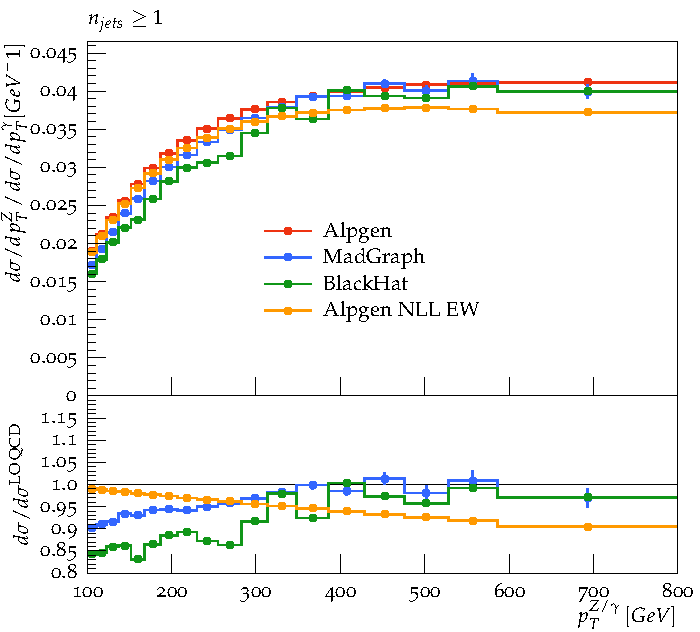
\includegraphics[width=0.49\textwidth]{d07-x01-y01-mc.pdf} \\
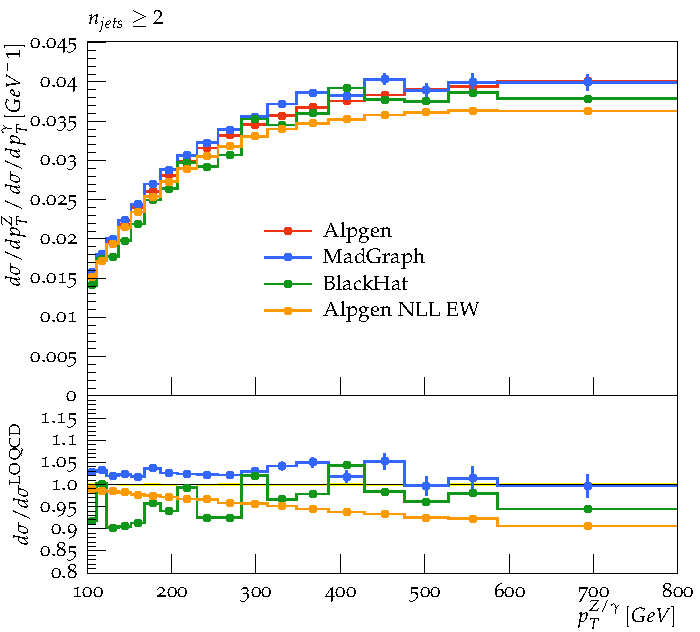
\includegraphics[width=0.49\textwidth]{d08-x01-y01-mc.pdf} \\
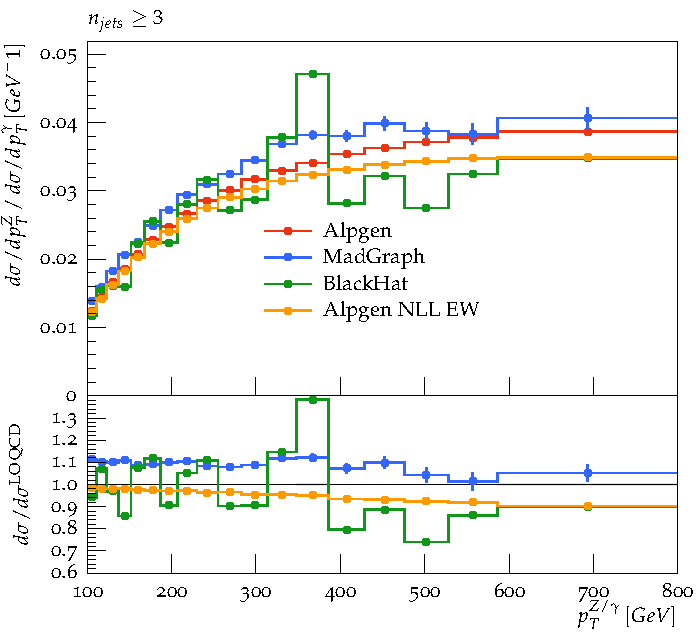
\includegraphics[width=0.49\textwidth]{d08-x02-y01-mc.pdf}
 \caption{Comparison of different predictions for the ratio of
   $\PZ+{}$jets over $\gamma+{}$jets at $8\UTeV$ pp 
   center-of-mass energy. From top to bottom, results are shown for events with at least 1, 2 and 3 jets accompanying the
   boson. For fixed-order predictions this value corresponds to the number of partons in the final state at the lowest order.}
\label{zgrmc}
\end{center}
\end{figure}
%
Figure~\ref{zgrmc} compares several predictions for the ratio within
the fiducial regions as defined above\footnote{We dropped the
  comparison for $H_{\mathrm{T}}>300\UGeV$ because fixed-order
  predictions are known to fail describing high jet activity with a
  comparatively low vector boson $p_{\mathrm{T}}$.}. The fixed-order
partonic predictions computed with the {\tt ALPGEN} generator are
shown at LO and at approximated NLO accuracy~\cite{Chiesa:2013yma},
i.e.\ including the effect of virtual weak corrections in the Sudakov
approximation obtained by means of the algorithm of
Refs.~\cite{Denner:2000jv,Denner:2001gw}, as described in Section
\ref{sec:sudakov;ew}. The predictions for $\PZ+{}$jets and
$\gamma+{}$jets are computed in the $G_{\mu}$ and $\alpha(0)$ schemes,
respectively, with the set of parameters listed above for the
calculation of the $\mathcal{O}(\alpha)$ corrections to the process
$\PW+2\,$jets. The factorization scale is set to $\sum_j
p_{\mathrm{T}}^j +\sqrt{M^2_V +p^2_{\mathrm{T},V}}$. CTEQ5L is used as
PDF set: it is worth noticing, however, that PDFs largely cancel in
the $\PZ/\gamma$ ratio as pointed out in Ref.~\cite{Ask:2011xf}.  More
precisely, the predictions for $\gamma+{}$jets and $\PZ+{}$jets are
computed by using the {\tt phjet} and {\tt zjet} packages,
respectively: at variance with the {\tt vbjet} package, where the
external vector bosons are produced on-shell, in {\tt zjet} the $\PZ$
boson decays in a fermion--antifermion pair including all the off-shell
and spin-correlation effects. These packages include only the QCD
contributions of order $\alpha_s^{n \, {\rm jets}} \alpha$ to the LO
predictions. Though the LO results for $\PZ+{}$jets include exactly
off-shell and spin-correlation effects, the Sudakov corrections are
obtained in the on-shell approximation by using the phase-space
mapping described in Ref.~\cite{Denner:2014ina}.

The other predictions are also shown in the CMS paper, where a
detailed description of the configuration used can be found. For
$\PZ+{}$jets and $\gamma+{}$jets generated with the {\sc
  Madgraph5}~\cite{MadGraph5} program, the LO multiparton
matrix-element calculation includes up to four partons in the final
state. The showering and hadronization, as well as the underlying
event, are modelled by {\sc PYTHIA6}~\cite{pythia6}. The events are
generated with the CTEQ6L1~\cite{CTEQ6} parton distribution functions,
and the ktMLM matching scheme~\cite{MatchingPaper} with a matching
parameter of $20\UGeV$ is applied.  In addition to these Monte Carlo
signal data sets, a NLO perturbative QCD calculation from the {\sc
  BLACKHAT} Collaboration~\cite{BlackHat} is available for a boson
accompanied by up to three jets. These calculations use
MSTW2008nlo68cl~\cite{MSTW} with $\alpha_{s}=0.119$ as the PDF set,
and the renormalization and factorization scales are set to
$\mu_{\mathrm{R}}=\mu_{\mathrm{F}}=H_{\mathrm{T}}+E_{\mathrm{T}}^{\mathrm{V}}$, where
$H_{\mathrm{T}}$ is the scalar $p_{\mathrm{T}}$ sum of all outgoing
partons with $p_{\mathrm{T}}>20\UGeV$ and
$E_{\mathrm{T}}^{\mathrm{V}}$ is defined as
$\sqrt{m_{\mathrm{Z}}^{2}+\left(p_{\mathrm{T}}^{\mathrm{Z}}\right)^{2}}$
and $p_{\mathrm{T}}^{\gamma}$, respectively, for $\PZ+{}$jets and
$\gamma+{}$jets.  In addition, the photons must satisfy the Frixione
cone isolation condition~\cite{Frixione}.

From the plot it is clear that both NLO QCD and EW corrections are
negative with respect to the fixed-order LO predictions. The NLO QCD
corrections are larger for lower transverse momentum of the bosons,
reaching a 15\% effect for $N_{\mathrm{jets}} \geq 1$. A fraction of
this effect seems to be included by {\sc Madgraph5} predictions, which
include higher-order real-parton emissions in the matrix-element
calculation. The EW corrections increase with the boson transverse
momentum, up to about 10\% for $p_{\mathrm{T}} > 600\UGeV$ in events
with at least one jet. Both QCD and EW corrections decrease for
larger jet multiplicities. It can be also noticed that the {\tt Madgraph}
prediction overshoots the NLO QCD ones for larger multiplicities.

\begin{figure}
\begin{center}
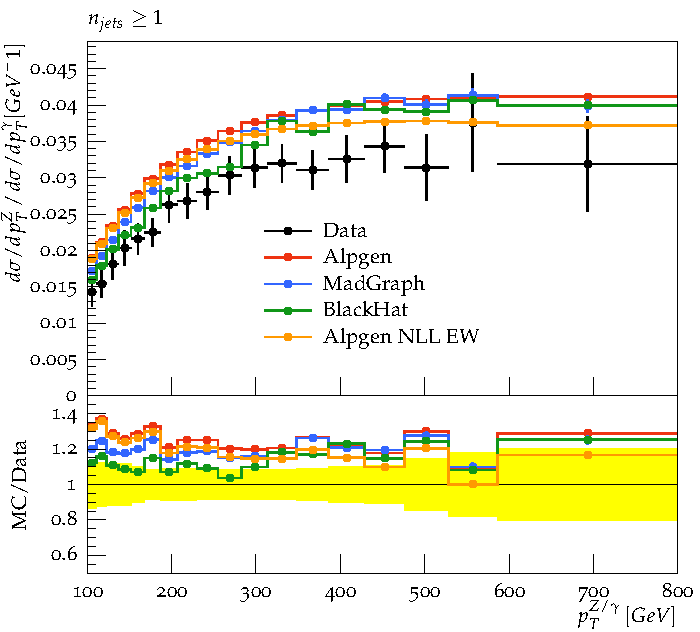
\includegraphics[width=0.49\textwidth]{d07-x01-y01.pdf} \\
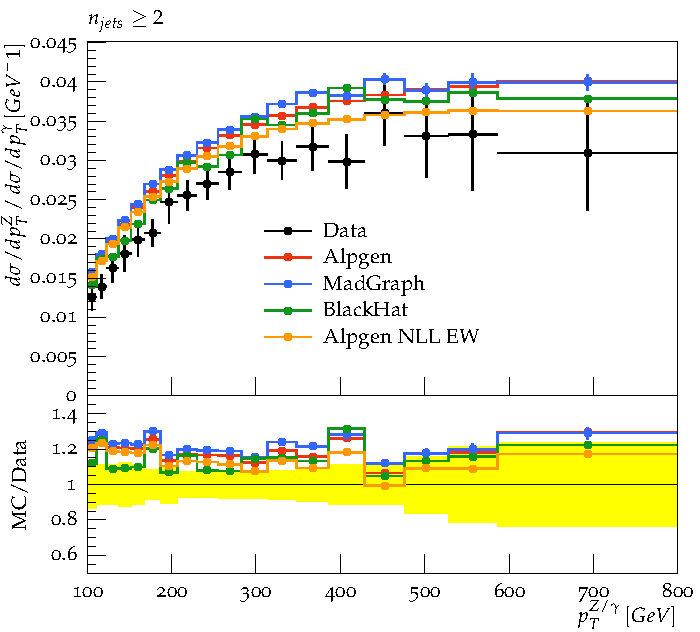
\includegraphics[width=0.49\textwidth]{d08-x01-y01.pdf} \\
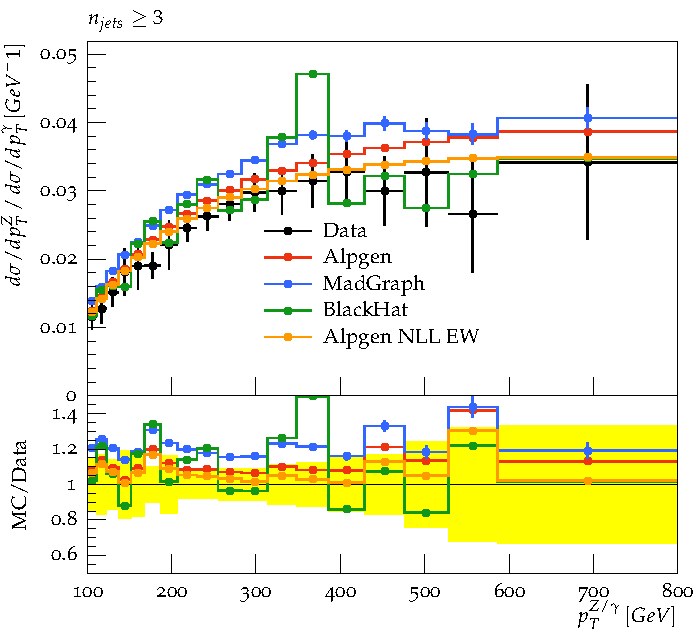
\includegraphics[width=0.49\textwidth]{d08-x02-y01.pdf}
 \caption{Comparison to CMS data of different predictions for the
   ratio of $\PZ+{}$jets over $\gamma+{}$jets at $8\UTeV$ pp 
   center-of-mass energy. From top to bottom, results are shown for events with at least 1, 2 and 3 jets accompanying the
   boson. For fixed-order predictions this value corresponds to the number of partons in the final state at the lowest order.}
\label{zgrdata}
\end{center}
\end{figure}
%
In Figure~\ref{zgrdata}, these predictions are compared to CMS
results, showing that the agreement improves when NLO corrections are
included, both in the case of QCD and EW ones. In particular,
including the EW corrections, results are in better agreement in the
region of high boson transverse-momenta, especially for larger jet
multiplicities.

\begin{figure}
\begin{center}
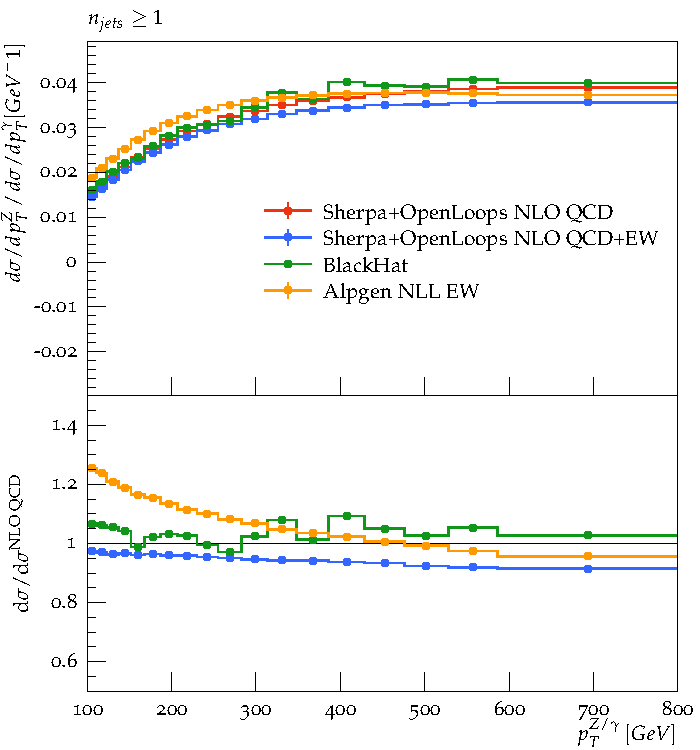
\includegraphics[width=0.5\textwidth]{d07-x01-y01-SherpaOL-mc.pdf} \\
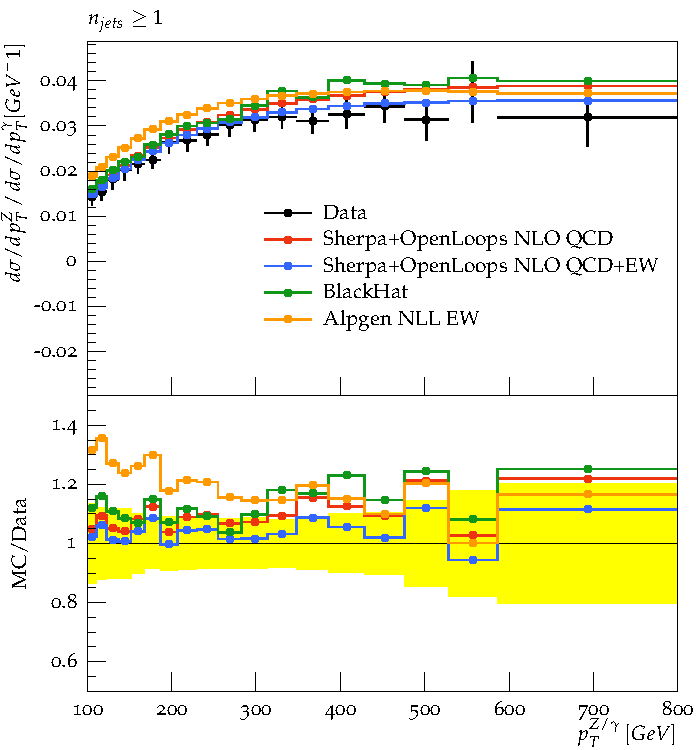
\includegraphics[width=0.5\textwidth]{d07-x01-y01-SherpaOL.pdf} \\
 \caption{Comparison of different predictions at NLO QCD,  NLL EW and
   NLO QCD+EW order for the  
   ratio of $\PZ+{}$jets over $\gamma+{}$jets at $8\UTeV$ pp
   center-of-mass energy, in events with at least 1 jet accompanying
   the boson. For fixed-order predictions this value corresponds to
   the number of partons in the final state at the lowest order. The
   top plot shows a comparison among the predictions, the bottom plot
   a comparison to CMS data. }
\label{zgrNLO}
\end{center}
\end{figure}
%
Finally, Figure~\ref{zgrNLO} shows in addition, for events with a
vector boson and at least one jet, fixed-order predictions from {\tt
  Sherpa+OpenLoops}. The $\PZ+{}$jets prediction is obtained from an
off-shell calculation for $\Pl^+\Pl^-+{}$jets including all
$\PZ/\gamma^*$ interference effects.  The presented predictions are
based on the recently achieved automation of NLO QCD+EW
calculations~\cite{Kallweit:2014xda,Kallweit:2015dum}, as described in
Section~\ref{sec:comp;ew}. Related predictions for the
$\PZ+{}$jets/$\gamma+{}$jets ratio (with an on-shell $\PZ$ boson) from {\tt
  Munich+OpenLoops} have already been presented
in Ref.~\cite{Kallweit:2015fta} and have for example been employed for
background predictions in Ref.~\cite{CMS:2015jdt}. Here, we employ
NNPDF2.3QED \cite{Ball:2013hta} parton distributions with
$\alpha_s=0.118$, and all input parameters and scale choices are as
detailed in Ref.~\cite{Kallweit:2015dum}. In particular, all unstable
particles are treated in the complex-mass scheme~\cite{Denner:2005fg},
and renormalization and factorization scales are set to
$\mu_{\mathrm{R,F}}=\hat{H}_{\mathrm{T}}'/2$, where $\hat{H}_{\mathrm{T}}'$ is
the scalar sum of the transverse energy of all parton-level
final-state objects, $\hat{H}_{\mathrm{T}}' = \sum_{i\in
  \{\mathrm{quarks,gluons}\}} p_{\mathrm{T},i} + p_{\mathrm{T},\gamma}
+ E_{\mathrm{T}, V}$. QCD partons and photons that are radiated at NLO
are included in $\hat{H}_{\mathrm{T}}'$, and the vector-boson
transverse energy, $E_{\mathrm{T},V}$, is computed using the total
(off-shell) four-momentum of the corresponding (dressed) decay
products, i.e.\
$E^2_{\mathrm{T},\PZ}=p^2_{\mathrm{T},\Pl\Pl}+m_{\Pl\Pl}^2$ and
$E^2_{\mathrm{T},\gamma}=p_{\mathrm{T},\gamma}^2$. The weak coupling
constant $\alpha$ is renormalized in the $G_{\mu}$ scheme for the
$\Pl^+\Pl^-+{}$jets prediction, while the $\alpha(0)$~scheme is used
for the $\gamma+{}$jets prediction. Results are presented at the NLO QCD
level and combining QCD and EW corrections via an additive
prescription, i.e.\ $\sigma^{\mathrm{NLO}}_{\mathrm{QCD+EW}} =
\sigma^{\mathrm{LO}}+\delta\sigma^{\mathrm{NLO}}_{\mathrm{QCD}} +
\delta\sigma^{\mathrm{NLO}}_{\mathrm{EW}}$. Isolated photons in the
$\gamma+{}$jets predictions are required to satisfy Frixione cone
isolation~\cite{Frixione} with parameters as specified in
Ref.~\cite{Khachatryan:2015ira}.

The agreement of the combined NLO QCD+EW prediction with the CMS data is
remarkable over the whole spectrum. As already noted, at low transverse momentum
NLO QCD corrections to the ratio are relevant due to mass effects, but sizable
EW corrections due to EW Sudakov logarithms (of different size for the two
processes) alter the shape of the ratio prediction already much below $1\UTeV$.
These results show the importance of combining NLO QCD and EW corrections in a
unified framework.






\subsection{Conclusions}
In this contribution we have performed a comparison of calculations of
EW corrections between different automated codes. While it is
a non-trivial task to precisely adjust the settings of the different
calculations such that they are consistent with each other,  we found a
typical agreement at the level of one per cent. We also compared the
Sudakov approximation to exact NLO calculations. Depending on the
considered process and the considered observable the Sudakov
approximation can describe the complete EW NLO corrections at the
level of one to ten per cent.
%
When comparing CMS data for the ratio of the associated production of a
$\PZ/\gamma^*$ or an on-shell photon with one or more jets to theoretical
predictions, the inclusion of EW corrections results in a better
agreement for high boson transverse momenta. 



\subsection*{Acknowledgements}
The work of A. Denner was supported by the Deutsche Forschungsgemeinschaft
(DFG) under reference number DE~623/2-1. 
%
The work of D. Pagani is supported  by the ERC grant 291377 ``LHCtheory: Theoretical predictions and analyses of LHC physics:
advancing the precision frontier''.
%
M. Zaro is supported by the European Union's Horizon 2020 research and
innovation programme under the Marie Sklodovska-Curie grant agreement
No 660171 and in part by the ILP LABEX (ANR-10-LABX-63), in turn
supported by French state funds managed by the ANR within the ``Investissements d'Avenir'' programme under reference
ANR-11-IDEX-0004-02.


\bibliography{ew_comparison}

\end{document}
